\documentclass[a4paper,man,floatsintext,natbib,donotrepeattitle, apacite]{apa6}
\usepackage{authblk}
\usepackage[utf8]{inputenc}
\usepackage{rotating} % provides sidewaystable and sidewaysfigure
\usepackage{natbib}
\bibliographystyle{apa}
\usepackage{bibentry}
\setcitestyle{notesep={; },round,aysep={},yysep={;}}
\usepackage[T1]{tipa}
\usepackage{amsmath}
\usepackage{enumitem}
\usepackage{makecell}
\usepackage{array}
\usepackage{float}
\usepackage{rotating}
\geometry{reset, letterpaper, height=9in, width=7in, hmarginratio=1:1, vmarginratio=1:1, marginparsep=0pt, marginparwidth=0pt, headheight=15pt}
\newcolumntype{P}[1]{>{\centering\arraybackslash}c{#1}}
\usepackage{bm}
\usepackage{tikz}
\usepackage{lmodern}
\usepackage{lipsum,ragged2e}% justify paragraphs
\usepackage{setspace}
\usepackage{endnotes} % put footnotes at end of paper
\usepackage{hyperref} % for urls

\let\footnote\endnote
\title{\LARGE Word structure in early Quechua speech}
\shorttitle{Early Quechua Speech}

\usetikzlibrary{shapes.geometric, arrows,backgrounds,fit,positioning}

\author[a]{\large Margaret Cychosz}

\affil[a]{\small University of California, Berkeley, Department of Linguistics, 1203 Dwinelle Hall, Berkeley, USA, \url{mcychosz@berkeley.edu}}
\affiliation{} % to remove weird affiliation

\abstract{Evidence from acoustic and articulatory phonetics suggests that linguistic structure is reflected in spoken language patterns. For child language, this interaction between word structure and speech production has the potential to shed considerable light on the status of children’s early word forms---but the topic remains underexplored in child speech. How is morphological structure reflected in children's speech? To answer this, the current study measured the speech patterns of bilingual Quechua-Spanish children (5-10 years) and adults. Coarticulation and duration were measured in two word environments, within morphemes and across morpheme boundaries. Both child and adult participants distinguished between the word environments, but they did so in different ways. Children differentiated between environments via distinct combinations of duration and coarticulation while adults consistently coarticulated more in shorter duration sequences. Additionally, the children’s speech patterns, but not the adults’, were sensitive to prosodic length: children produced increasingly shorter phones in words with more syllables. It is suggested that the differences between adults and children are attributable to adults' faster speaking rate and increased dominance in Quechua.}

\keywords{coarticulation; acoustics; morphology; field phonetics; first language acquisition; Quechua}


\clearpage

\begin{document}
\justifying
\setlength\parindent{24pt} % indent each paragraph

\maketitle

\setcounter{secnumdepth}{2} % number sections


\section{Introduction}

Adult speakers can readily compose novel, morphologically complex word forms like \textit{daxy} or \textit{unraxlike} from morphemic subcomponents. Evidence of u-shaped learning curves in children, and the results of \citet{berkoChildLearningEnglish1958}'s Wug Test, have led developmental researchers to recognize that young children must share in adults' morphological productivity. If not, children would not be able to extend morphophonological patterns, such as the correct plural allomorphs, to novel lexical environments. Yet there remains disagreement concerning children’s early linguistic representations: researchers disagree about when children begin to analyze the internal structure of words that---at least for adults---are complex. Children's lexical forms could be fully adult-like from early toddlerhood (e.g., \citealt{wexlerVeryEarlyParameter1998}) the forms could emerge over time with usage (e.g., \citealt{ambridgeUbiquityFrequencyEffects2015}), or there could be some combination of the two approaches (e.g., \citealt{swingleyLexicalNeighborhoodsWordForm2002}). 

There are factors, beyond the ability to flesh out a morphological paradigm with novel forms, that reveal whether children have adult-like production mechanisms for complex words. One window into the nature of lexical access and storage---at least in adult speakers---is to examine the effects of morphological structure on speech production. Adults, and even children, have been shown to produce complex words differently, arguably as a result of planning differences, or maybe practice (\citealt{choEffectsMorphemeBoundaries2001}; \citealt{hayCausesConsequencesWord2003}; \citealt{lee-kimMorphologicalEffectsDarkness2013}; \citealt{plagPhonologicalPhoneticVariability2014}; \citealt{songDurationalCuesFricative2013}; \citealt{songEffectsCoarticulationMorphological2013};  \citealt{strycharczukPhoneticDetailPhonetic2019}; \citealt{sugaharaDurationalCorrelatesEnglish2009}; 
\citeauthor{tomaschekHowAnticipatoryCoarticulation2019} \textit{under review}). For example, in adult speech, morphologically complex words like \textit{sighed} can be longer in duration than their simplex counterparts like \textit{side} \citep{sugaharaDurationalCorrelatesEnglish2009}. And children have been shown to coarticulate more between adjacent segments within mono-morphemic words like \textit{box} than between otherwise identical segments that straddle a morpheme boundary as in \textit{rocks} \citep{songEffectsCoarticulationMorphological2013}. 

This study takes advantage of hypothesized relationships between acoustics, specifically coarticulation and duration, and word structure. The complex relationship between speech variability and linguistic structure is still relatively underexplored in children and adults (cf. \citealt{redfordGrammaticalWordProduction2018}; \citealt{songDurationalCuesFricative2013}; \citealt{songEffectsCoarticulationMorphological2013}). Yet measuring how morphological structure is reflected in children's speech could allow us to infer about the status of children's early complex word forms. Are words that, to an adult are transparently morphologically complex, treated as such by children? And when a child does recognize that a given word is morphologically complex, how does this recognition affect children's speech production? 

To that end, the goal of this study is to evaluate how the composition of morphologically complex words is reflected in children's speech production patterns in Quechua, a highly agglutinating language with over 200 productive verbal and nominal suffixes. In doing so, this work follows a still-developing line of research that evaluates relationships between linguistic structure and speech production (e.g., \citealt{hayCausesConsequencesWord2003}; \citealt{plagPhonologicalPhoneticVariability2014}; \citealt{songEffectsCoarticulationMorphological2013}; \citealt{songDurationalCuesFricative2013}, \citealt{strycharczukPhoneticDetailPhonetic2019}; \citeauthor{tomaschekHowAnticipatoryCoarticulation2019} \textit{under review}). Here, coarticulation, and its relationship with duration, is measured across and within morpheme boundaries in adults and a cross-sectional cohort of school-aged children to examine if, and how, Quechua speakers distinguish between morphological environments in their speech. It is anticipated that children, who have less experience with language and potentially less abstract linguistic representations, will coarticulate similarly within between and within morpheme boundaries. This behavior would suggest that the children are not as likely as adults to analyze the internal structure of complex word forms. Adults, however, will distinguish between morphological environments in their speech because they analyze the internal structure of complex words and compose these words together from the component morphemic parts.

The choice to study these patterns by prosodic environment in a highly agglutinating language like Quechua is an important one. Quechua may make an important typological contribution to this literature because, given the complexity of its word forms, there are few doubts as to children's productivity from a very young age \citep{courtneyLearningConstructVerbs2002}. Furthermore, the sheer number of available inflectional forms in Quechua, compared to more analytic languages such as English, likely translates into less competition between forms accessed in their inflected form and those composed online from individual morphemes during word retrieval (\citealt{hayCausesConsequencesWord2003}; \citealt{pinkerFutureTense2002}). In short, evidence that children are not distinguish between the two morphological environments could be especially noteworthy in a language of this structure.  

\section{Background}

\subsection{Accessing complex words}

Adult speakers’ ability to compose novel, morphologically complex words (e.g., \textit{twinkly}) appears to be highly flexible and abstract. Children’s early overgeneralization errors (e.g., \textit{I taked*}) demonstrate how even very young speakers analyze the internal structure of words and apply morphemes in new, unheard environments. Consequently, morphological productivity is a defining characteristic of the language faculty after a certain point in development. 

Still, there is some behavioral evidence that adult speakers do not uniformly decompose complex words \citep{taftLexicalStorageRetrieval1976}. 
Using lexical frequency statistics, some work suggests that adults may instead access complex words, especially high-frequency complex words, holistically in the mental lexicon, without decomposing them (\citealt{baayenQuantitativeAspectsMorphological1992}; \citealt{baayenFrequencyEffectsRegular2003}). For example, \citet{coleWordsMorphemesUnits1997} tested this idea and demonstrated a processing advantage for high-frequency base stems (e.g., \textit{fish}) versus derived words (e.g., \textit{fisher}). Crucially, this advantage diminished when the derived word was more frequent than the base stem. 

\citet{hayCausesConsequencesWord2003} likewise demonstrated relative frequency effects. Measuring speech production (contrastive pitch accent placement and phonetic reduction at morpheme boundaries), Hay showed that when derived words are more frequent than their corresponding base form (e.g., \textit{disentangle} vs. \textit{entangle}), these words may be accessed holistically (see \citealt{pluymaekersMorphologicalEffectsFine2010} for an alternative explanation). Similarly, greater root frequency relative to a suffix is usually predictive of decomposition, at least in more analytic languages \citep{smithPhoneticDetailThat2012}. And less frequent words, or words that only occur with a given suffix, do not necessarily manifest complete morphological decomposition \citep{kempsProsodicCuesMorphological2005}. 
\citet{hayCausesConsequencesWord2003}'s findings in particular imply a dual-route model of complex word access, where two different lexical mechanisms---holistic storage and online complex word formation---compete during complex word production (\citealt{baayenQuantitativeAspectsMorphological1992}; \citealt{koenigTypeUnderspecificationOnline1995}; \citealt{pinkerRegularIrregularMorphology1994}; \citealt{pinkerFutureTense2002}). The method of construction that is fastest, predicted by the relative frequency of base to derived form, wins. 

Finally, a number of computational models have attempted to predict decomposition versus whole-word storage. In a model of English morphology, \citet{ingoplagSuffixOrderingMorphological2009} demonstrated that affixes that are highly parsable---affixes that speakers can more easily separate from their root (e.g., English -\textit{ness})---predict decomposition. Affixes that are highly fused to the stem---those that speakers are less able to parse from the stem (e.g. English -\textit{th})---predict whole-word access. And more recently, \citet{odonnellProductivityReuseLanguage2015} proposed a probabilistic model where speakers weigh the productiveness of rules versus the storage of idiosyncratic, complex words to predict decomposition. 

Given children's u-shaped learning curves, and their performance on the Wug test \citep{berkoChildLearningEnglish1958}, it is often assumed that children as young as four years share adults' morphological productivity capacities. Consequently, the above findings that cast doubt upon whether composition is always the online strategy that wins during lexical access for \textit{adults} are highly relevant to the study of how children access morphologically complex words. Frequency ratios appear to predict word (de)composition in adults (e.g., \citealt{hayCausesConsequencesWord2003}). Thus, since frequency ratios change as children learn more words, stems, and suffixes, one can predict that the fastest manner for children to access a complex word---by composition or holistic access---will also change over the course of development. But lexical frequency ratios are just one method to evaluate complex word access. Another method may be to evaluate how children, particularly a cross-sectional cohort of children spanning several years of development, reflect morphological structure in their speech throughout development. This is the objective of the current study. 

\subsection{Morphological structure and speech production}

One way to study how speakers analyze complex words, and access them in the mental lexicon, is to measure the effect of morphological structure on speech production. \textsc{Morphophonetics}, or how morphological structure manifests in fine, phonetic variability, is increasingly studied in adult speech, though the results are not always conclusive (see \citet{plagPhonologicalPhoneticVariability2014} and \citet{strycharczukPhoneticDetailPhonetic2019} for recent overviews). Researchers now know that morphological structure and composition dictates \textit{some} speech variability in adults (\citealt{choEffectsMorphemeBoundaries2001}; \citealt{guyExplanationVariablePhonology1991}; \citealt{hayCausesConsequencesWord2003};
\citealt{lee-kimMorphologicalEffectsDarkness2013}; \citealt{plagHomophonyMorphologyAcoustics2017}; \citealt{smithPhoneticDetailThat2012}; \citealt{sugaharaDurationalCorrelatesEnglish2009}; \citeauthor{tomaschekHowAnticipatoryCoarticulation2019} \textit{under review}; cf. \citealt{haniqueRoleMorphologyAcoustic2012}), but it is often unclear when, how much, or even why (\citealt{mousikouMorphologicalEffectsPronunciation2015}; \citealt{plagPhonologicalPhoneticVariability2014}).

~
~
\subsubsection{Adult speech}

One of the earliest studies to examine the relationship between phonetics and word structure was \citet{losiewiczWordFrequencyEffects1995} who found that frequency affected the phonetic realization of morphemes. Specifically, English past tense -\textit{ed} was temporally longer on low-frequency verbs than high-frequency verbs.\footnote{Recent statistical advances have called into question the results of \citet{losiewiczWordFrequencyEffects1995} (see \citet{seyfarthAcousticDifferencesMorphologicallydistinct2018}).}. 
Elsewhere, \citet{sugaharaDurationalCorrelatesEnglish2009} found that heteromorphemic words were longer than otherwise identical monomorphemic words (e.g. \textit{sighed} versus \textit{side}), while \citet{smithPhoneticDetailThat2012} found that pseudo-prefixes (\textit{mistake}) were shorter in duration than real prefixes (\textit{misjudge}). Finally, \citet{seyfarthAcousticDifferencesMorphologicallydistinct2018} examined paradigmatic influences on segmental duration in English, for example predicting differences between \textit{frees} and \textit{freeze} based on membership in the \textit{free} paradigm. After controlling for lexical frequency, prosodic structure, and orthography, the authors found that paradigm membership can sometimes predict segment duration, though this depends upon the segment studied (fricatives versus stops). 

Articulatory methods have likewise been used to evaluate the relationship between morphology and phonetic variation in adult speech. \citet{choEffectsMorphemeBoundaries2001} found that intergestural timing in Korean, measured with electromagnetic articulagraphy and electropalatography, was more stable within a word than across a morpheme boundary. The author found a similar effect for a lexicalized compound word versus a non-lexicalized compound word (noun phrase). In addition, English /l/ darkness has been found to vary by position at morphological boundaries \citep{lee-kimMorphologicalEffectsDarkness2013}. The phone /l/ is darker in stem-final position (\textit{coolest}) than affix–initial (\textit{coupless}), independent of duration, because \textit{coolest} is analogizing to word-final /l/ in its base form \textit{cool} (See also \citealt{strycharczukGradualAbruptPhonetic2016}). Most recently, \citeauthor{tomaschekHowAnticipatoryCoarticulation2019} (\textit{under review}) measured anticipatory coarticulation patterns in English. The authors used electromagnetic articulagraphy to evaluate the degree of morphological opacity in inflected verbs. Results showed that English speakers exhibited greater anticipatory coarticulation of the vowel in a verb stem (e.g., \textit{clean}) for those verb inflections with which they had increased experience and practice. 

However, the relationship between speech production and morphology is not always straightforward. Morphological structure, and morphologlical analysis, co-varies with a number of other measures including orthography, frequency, and prosodic structure. For example, \citet{plagHomophonyMorphologyAcoustics2017} found that, after controlling for a host of other factors such as number of syllables, speaking rate, and surrounding context, the duration of English /s/ and /z/ varied systematically by morphological status. But the morphemic plural and non-morphemic /s, z/ were longer in duration than morphemic /s, z/ used as third person markers. The cause of this difference is not clear, though some authors suggest that the spontaneous speech analyzed in \citet{plagHomophonyMorphologyAcoustics2017} may explain the findings \citep{seyfarthAcousticDifferencesMorphologicallydistinct2018}. Elsewhere, others have argued that it is not morphological structure but word information load (\citealt{haniqueRoleMorphologyAcoustic2012}; \citealt{pluymaekersMorphologicalEffectsFine2010}) or contextual predictability \citep{cohenProbabilisticReductionProbabilistic2014} that explains these interactions between speech production and word structure. 

A complete  review on the consequences of morphological structure for adult speech production is beyond the scope of a paper on children's speech development. What is important, however, is that the previous two decades of morphophonetics research has converged somewhat on the fact that words with productive morphology are produced differently than simplex words (\citealt{kempsProsodicCuesMorphological2005}; \citealt{plagPhonologicalPhoneticVariability2014}; \citeauthor{tomaschekHowAnticipatoryCoarticulation2019} \textit{under review}). For child speech, these findings present a new method to detect when and whether children are decomposing words. Furthermore, the current work extends the study of morphophonetics to Quechua. This could be an important typological contribution not just because Quechua's morphology is highly productive, but because Quechua's agglutinating structure means that there should be less relative frequency effects between forms composed online and those accessed in the inflected form (\citealt{baayenQuantitativeAspectsMorphological1992}; \citealt{hayCausesConsequencesWord2003}; \citealt{pinkerFutureTense2002}). 

Consequently, the goal of this paper is twofold. First, it extends the hypothesized relationship between speech production and morphological structure to a new participant sample that includes adults and a large cross-sectional sample of children. Second, it examines production and morphological structure in a language with a vastly different word structure from the western European languages that have been the focus of previous research.   

~
~

\subsubsection{Child speech}\label{child-morph}

While we understand some of the explanatory mechanisms behind morphological structure and phonetic variation in adult speech, this relationship is less studied in children (cf. \citealt{songDurationalCuesFricative2013}; \citealt{songEffectsCoarticulationMorphological2013}). As a developing sub-area in phonetics, morphophonetics has the potential to inform our understanding of the structure of the mental lexicon throughout development. For the current study, examining child morphophonetics also contributes to a line of research evaluating the status of children's early word forms:  some theorists posit that children's lexical forms are fully adult-like from early toddlerhood (e.g., \citealt{wexlerVeryEarlyParameter1998}), while others posit that they emerge over time with usage (e.g., \citealt{ambridgeUbiquityFrequencyEffects2015}), or a combination of the two approaches (e.g., \citealt{swingleyLexicalNeighborhoodsWordForm2002}). 

A handful of studies have examined how morphological structure is reflected in children's speech to address the question of how children represent complex words. \citet{songEffectsCoarticulationMorphological2013} studied this in English-learning children. They employed acoustic and ultrasound analyses to study adult and 2;0 (year;month) children’s CC syllable (/ks/) coarticulation in the coda of bimorphemic (\textit{rocks}) and monomorphemic (\textit{box}). (These, along with \textit{rock} and the nonword \textit{das}, were the items tested.) The articulatory data showed that children reliably raised their tongue more for \textit{rocks} than \textit{box}, suggesting that they could distinguish between morphemic and non-morphemic coda consonant clusters. While there was no evidence of anticipatory coarticulation for \textit{box} in the adults or children studied, there was a strong perseveratory coarticulation effect of /k/ on /s/ in \textit{box} and anticipatory coarticulation effect of /s/ on /k/ in \textit{rocks}. This finding led the authors to conclude that the primary articulatory target for monomorphemic \textit{box} was the C\textsubscript{1} of the consonant cluster (/ks/), while the articulatory target for bimorphemic \textit{rocks} was C\textsubscript{2} or the plural morpheme /s/. The articulatory target differs by morphological role, suggesting that semantic information may be encoded in articulatory gestures. This applied for both adults and children.

Elsewhere, coda position American English fricatives /s, z/ were studied in the naturalistic speech of children and their caretakers \citep{songDurationalCuesFricative2013}. Children’s morphemic /z/ was longer in duration than non-morphemic /z/ in word-final position. This acoustic evidence suggests that, as early as 2;0, child speakers of American English reliably distinguish between otherwise identical morphemic and non-morphemic segments. The authors used this finding to argue that even at this young age children may not rote-memorize morphologically complex forms, but may instead compose the words online.

Finally, \citet{redfordGrammaticalWordProduction2018} studied the relationship between word structure and phonetic variation across word boundaries in prosodic words (e.g., \textit{the bat}). The results showed that /\textschwa/ in children's \textit{the} productions were reliably louder and longer than in adults' productions. According to Redford, this result was strong evidence that children exhibit immature timing control, but the results were inconclusive concerning children's speech organization---whether children accessed the prosodic words holistically or in parts.

These developmental studies aside, the relationship between speech production and morphological structure is infrequently explored in children. This is to the detriment of the field because a parallel line of research on children's coarticulation has shed considerable light on early phonological representations. Conflicting evidence from this research suggests that children may store speech and word forms in larger chunks than adults, at the syllabic level or higher (e.g., \citealt{nittrouerEmergencePhoneticSegments1989};  \citealt{noirayBackFutureNonlinear2019}; \citealt{zharkovaCoarticulationIndicatorSpeech2011}). The following section summarizes this work.

\subsection{Children's phonological storage: Evidence from coarticulation}\label{child-coartic}

Numerous works have found that children coarticulate more than adults, often until early puberty, with the degree and variability of coarticulation decreasing with age (\citealt{goodellAcousticEvidenceDevelopment1992}; \citealt{nittrouerEmergencePhoneticSegments1989}; \citealt{nittrouerHowChildrenLearn1996}; \citealt{noirayBackFutureNonlinear2019};  \citealt{zharkovaSpatialTemporalLingual2014}; \citealt{zharkovaDynamicsVoicelessSibilant2018} \textit{inter alia}). Many authors have interpreted this relationship between coarticulation and age as evidence that young children represent speech in syllable-sized units, which gradually individuate into phoneme-sized units over the course of development. 

While one may expect children to coarticulate less than adults---children speak slower and with less coordinated movement \citep{smithRelationshipsDurationTemporal1992}---many studies have concluded that children coarticulate \textit{more} than adults (\citealt{goodellAcousticEvidenceDevelopment1992}; \citealt{nittrouerEmergencePhoneticSegments1989}; \citealt{nittrouerHowChildrenLearn1996};  \citealt{zharkovaCoarticulationIndicatorSpeech2011}). Citing this evidence, some have argued that the phenomenon of ``coarticulation'' in child speech reflects children's phonological representations (this will be outlined in further detail in the following section). This approach thus argues that unlike adult coarticulation, child coarticulation does not necessarily reflect efficiency in speech planning or the clear anticipation of upcoming segments ( \citealt{bradlowConfluentTalkerListeneroriented2002}; \citealt{whalenCoarticulationLargelyPlanned1990}), but instead reflects a larger representational unit. 

Studying children's coarticulation, \citet{nittrouerEmergencePhoneticSegments1989} concluded that children may have more holistic, syllable-sized representations. The authors measured coarticulation in fricative-vowel sequences within nonce words to test the anticipatory effect of vowels on /s/ and /\textesh/. Their results from children 3;0-8;0 showed that children coarticulated more than adults---vowels affected the children's fricative production more than the adults' production. This led the authors to conclude that this pattern manifested in the fricative-vowel sequences because the children did not distinguish between /s/ and /\textesh/ as reliably as the adults. It was not, the authors argued, because children differed from adults in their degree of anticipatory lip rounding or even the lingual constriction shape (see also \citealt{nittrouerHowChildrenLearn1996}).

\citet{nittrouerEmergencePhoneticSegments1989}'s findings partially supported conclusions from the two children studied in \citet{reppObservationsDevelopmentAnticipatory1986}. There, the younger child (4;8) showed greater anticipatory lip rounding for /s/ before /u/ than the older child (9;5). More recently, the coarticulation patterns of children with and without apraxia of speech and adults without apraxia were studied \citep{nijlandCoarticulationPatternsChildren2002}. Participants produced nonce sequences of \textschwa-V-C where V was /a, \textsci, or u/ and C was /s, x, b, or d/. The typically-developing children once again showed more intra- and inter-syllabic anticipatory coarticulation than the adults.

Most recently, Zharkova and colleagues (\citealt{zharkovaCoarticulationIndicatorSpeech2011}; \citealt{zharkovaSpatialTemporalLingual2014}; \citealt{zharkovaDynamicsVoicelessSibilant2018}) and Noiray and colleagues (\citealt{noirayHowChildrenOrganize2018}; \citealt{noirayBackFutureNonlinear2019}; \citealt{rubertusDevelopmentGesturalOrganization2018}) incorporated articulatory ultrasound data and have frequently observed that children coarticulate more than adults. The authors frequently infer that children's propensity to coarticulate reflects their larger representational units. In \citet{zharkovaCoarticulationIndicatorSpeech2011}, children aged (6;3-9;9) altered their productions of /\textesh/ based on the following vowel (/a, i, or u/) more than adults. However, \citet{zharkovaSpatialTemporalLingual2014} conducted a similar experiment with older children (10;0-12;4) and did not find any differences between child and adult coarticulation patterns. The authors suggest that children may approximate adult-like phonological representations by preadolescence. 

Also using ultrasound imaging, \citet{noirayBackFutureNonlinear2019} measured vocalic anticipation in children (3;05-7;06) and adults. They found that in V\#CV strings, children anticipated the upcoming vowel sooner than adults at age 3;0 and 5;0, but progressively less by 7;0. (See \citet{noirayHowChildrenOrganize2018} for segment-specific explanations for coarticulation development.) Most recently, \citet{noiraySpokenLanguageDevelopment2019} correlated children's (4;06-7;02) coarticulation, measured articulatorily with ultrasound imaging, with measures of expressive vocabulary and phonological awareness. The amount of children's intrasyllabic coarticulation and gestural individuation was negatively correlated with phonological awareness (a measure of speaker awareness of segmental units), which the authors suggest reflects a lack of segmental individuation in children. 

Authors of the above acoustic and articulatory studies often argue that children's coarticulation patterns reflect holistic, syllable-sized representations. According to such an interpretation, representations progressively individuate and become more adult-like as children age. It is nevertheless important to note that results in the child coarticulation literature are mixed. Numerous studies have instead found that adults coarticulate more than children. These works often argue that children's phonological representations are just as or more discretely organized into individual segments than adult phonology. As a result, children learn to coordinate and exhibit appropriate coarticulatory overlap as part of standard phonetic and/or phonological development (\citealt{barbierSpeechPlanningIndex2013}; \citealt{barbierSpeechPlanning4yearold2015}; \citealt{katzAnticipatoryCoarticulationSpeech1991}; \citealt{kentSegmentalOrganizationSpeech1983}; \citealt{whitesideSpeechPatternsChildren2000}). Other works have found no differences in coarticulatory patterns between adults and children (\citealt{flegeAnticipatoryCarryoverNasal1988}; \citealt{goffmanBreadthCoarticulatoryUnits2008}; \citealt{noirayDevelopmentMotorSynergies2013}; \citealt{serenoDevelopmentalAspectsLingual1987}; \citealt{serenoAcousticAnalysesPerceptual1987}).

Methodological differences between the studies summarized above may account for some of the different conclusions concerning children's coarticulation patterns. But the objective of this study is not to determine whether children coarticulate more or less than adults. Instead, evidence from the child coarticulation literature is summarized because it 1) suggests that children may initially represent speech more holistically in syllable- or word-sized units and 2) highlights the different approaches to measuring coarticulation in child speech. Even in child populations where data collection techniques are often more limited, there are innumerable techniques to measure coarticulation (e.g., acoustic [\citealt{nittrouerHowChildrenLearn1996}] or articulatory [\citealt{zharkovaSpatialTemporalLingual2014}]). But even within the acoustic realm there are different approaches. Most frequently, for fricatives, coarticulation is quantified as the change in centroid (average) based on vocalic context while coarticulation within vowels is typically quantified as the midpoint or steady-state formant value (\citealt{nittrouerEmergencePhoneticSegments1989}; \citealt{nittrouerHowChildrenLearn1996}). Elsewhere, coarticulation has been measured acoustically as the spectral change between adjacent segments (\citealt{gerosaAnalyzingChildrenSpeech2006}).

The current study employs one of these measures of spectral change, outlined in \citet{gerosaAnalyzingChildrenSpeech2006} and validated in \citet{cychoszSpectralTemporalMeasures2019}. This measure takes into account change occurring over the timecourse of segments, instead of static measurements. Children speak slower than adults, so taking measurements from the steady-state or midpoint of a vowel is not ideal. Children's slower speaking rate permits them greater opportunity to achieve a steady acoustic signature. Measuring coarticulation from a larger portion of the overall segment, which is what is proposed here, mitigates the effect of speaking rate to a certain degree.

\section{Current study}

\subsection{The language}\label{the-language}

The current study measures speech production across different morphological environments in South Bolivian Quechua, henceforth Quechua, a Quechua-II/C language with over 1.6 million speakers in southwest Bolivia and northwest Argentina \citep{toreroDialectosQuechuas1964}. This variety of Quechua is spoken in the Chuquisaca department of southern Bolivia. Like many Quechuan varieties, Quechua in southern Bolivia has been in intense contact with Spanish for hundreds of years resulting in large amounts of language mixing and borrowing (\citealt{muyskenContactsIndigenousLanguages2012}; \citealt{muyskenSpanishAffixesQuechua2012}). Furthermore, public schools in Bolivia are conducted primarily in Spanish. Consequently, almost all school-age children who speak Quechua in the home, such as the children in the present study, are bilingual in Spanish. And because of Spanish schooling, children in Bolivia learn to read in Spanish. Though Quechua has an established writing system, children generally do not learn to read or write in Quechua and few Quechua speakers use the language in its written form.

Quechua is a highly-agglutinating language with over 200 productive nominal and verbal suffixes that encode argument structure and grammatical relations (for comparison, English has around 35 productive suffixes). The morphology is nevertheless highly regular and not subject to significant morphophonological processes or fusion. The phonological inventory includes three phonemic vowels /i, a, u/ and two allophonic vowels derived in uvular contexts [e, o] \citep{gallagherVowelHeightAllophony2016}. The consonantal inventory contrasts voiceless stops, aspirated stops, and ejectives along four places of articulation, /p, t, k, q/, as well as a three-way alveopalatal stop-aspirated stop-ejective distinction /\textteshlig, \textteshlig\textsuperscript{h}, \textteshlig'/. Nasals are contrasted along three places of articulation, /m, n, \textltailn/ with an allophonic velar nasal. See Appendix \ref{app:app-A} for a complete consonant inventory. 

~
~

\subsection{Research objectives}

The primary objective of this paper is to measure how Quechua word structure affects speakers' production of morphologically complex words. To accomplish this, a relatively novel acoustic measure of coarticulation is employed, which has been validated for young children’s voices and a variety of consonants \citep{cychoszSpectralTemporalMeasures2019}. Using this measure, the coarticulation patterns in adult and child Quechua speakers are evaluated to see if, and how, the patterns differ between children and adults, and across development, in a cross-sectional sample of school-aged children. 

As an agglutinating language, Quechua provides unique insight into interactions of morphological structure and phonetics. Quechua speakers appear to have highly flexible inflectional and derivational lexicons: suffixes and roots are abstracted away from the original lexical contexts and are easily rearranged for novel stem+suffix pairings. This process is similar to how speakers of more analytic languages, such as English, effortlessly arrange novel noun-adjective pairings. It is this morphological structure that makes Quechua an interesting typological contribution to a study on phonetics and word structure. For one thing, as noted in the previous sections, given the number of possible complex word forms, is difficult to doubt the the morphological productivity of young Quechua speakers. Quechua is understudied, both in child language research and linguistics more broadly. Still, much like well-studied, less synthetic languages, there is undeniable evidence of morphological productivity in children's speech (and other highly agglutinating languages). Child speakers of Cuzco Quechua appear to have a productive morphology by age 5;0, if not earlier \citep{courtneyLearningConstructVerbs2002}.\footnote{Cuzco Quechua and South Bolivia Quechua are distinct varieties, but they are mutually-intelligible. There should be no reason to assume that children's morphological productivity would vary greatly between them.} 

Another reason why Quechua makes an important typological contribution again concerns its morphological structure. In Quechua, frequency ratios between words that might be compiled online and those that might be accessed holistically are likely to be much smaller. This also means that the type frequency of each word is lower than in moderately synthetic languages, like English and Dutch, which are more commonly studied in morphophonetics. So concerns about a race between online compilation and holistic access may be less relevant. 

One final reason why Quechua may be an interesting addition to the morphophonetics literature concerns its applied use in Bolivia. As described in section \ref{the-language}, very few Quechua speakers read or write in the language (speakers who attend school instead become literate in Spanish). Disengaging prosodic effects from orthographic effects has been immensely difficult for morphophonetics, and the study of phonetics in general (\citealt{seyfarthAcousticDifferencesMorphologicallydistinct2018}; \citealt{warnerOrthographicVsMorphological2006}). Quechua removes this problematic variable because speakers do not have strong orthographic representations.\footnote{Concerning Quechua orthography, it is important to emphasize two things. First, there \textit{is} a standardized, written form of South Bolivian Quechua. For example, students who study Quechua at the university level learn to read and write in the language and \textit{some} textbooks for school-aged children contain some words written in Quechua. Second, in my fieldwork, I have found that speakers certainly can write in Quechua, because the orthography is relatively transparent and Quechua shares many phonological characteristics with Spanish (e.g., five vowel system). But I have found this to be uncommon in the communities where I work.} Thus, while the primary typological interest of Quechua concerns its morphological productivity and what that means for the structure of the lexicon, there are additional, applied considerations that make Quechua a unique language to examine the effects of word structure on speech production. 

Given these characteristics of Quechua, this study makes two predictions. First, relying on the developing literature documenting effects of word structure upon speech production in children and adults, this study predicts that children will produce complex words differently from adults. The hypothesis is tested in a tightly-controlled experimental paradigm where coarticulation between the phones [a] and [p], or [a] and [m], is measured. The prediction is that adults, and potentially older children, will distinguish between the VC sequences that fall within morphemes (e.g., lla\textbf{ap}a `lightning’) and between morphemes (e.g., p\textbf{ap}a `potato’). The second prediction of this study is that children will coarticulate more than adults at morpheme boundaries meaning that overall, adults will show a larger differential between within- and across-morpheme coarticulation than children.

If older speakers' phonetic realization of the exact same [ap] or [am] sequence differs within a morpheme versus across a boundary, then we can infer that the adults are breaking words down at constituent boundaries: they have learned to parse speech segmentally and store it morphophonemically. The relative lack of distinction in the children's speech, however, infers that children may be accessing complex words in larger, inflected chunks whose internal structure the children may not have analyzed.

The predicted outcomes of this experiment do not suggest that Quechua-speaking children are morphologically unproductive. Instead of suggesting a lack of productivity, the predictions reflect recent proposals in child speech and language research that children may initially analyze language differently than adults and, as a result, children may store language more holistically (\citealt{davisEmergenceDiscretePerceptualMotor2019}; \citealt{lievenLexicallybasedLearningEarly1997};  \citealt{redfordSpeechProductionDevelopmental2019}). Such proposals argue that children do not always recognize complex forms as having an internal structure, and thus do not deconstruct words into morphemes, or morphemes into phones. Instead, children may be more prone to represent and access language in chunks, particularly frequently-occurring combinations or phonotactically-probable “subwords.” You could imagine that chunks in English, like \textit{Immagonna} or \textit{lookatit}, could be stored in this way, in addition to their deconstructed forms (individual words, morphemes, and phonemes). Thus, child language may be redundant, with representation at multiple levels in the grammar.

This approach to speech and language development may surprise some audiences---after all the birth of modern linguistics marked a decided turn away from memorized, holistic chunks (\citealt{chomskyReviewBFSkinner1959}; \citealt{skinnerVerbalBehavior1957}). This is because Behaviorism made untenable demands on psycholinguistic representation and instigated logical fallacies such as the Poverty of the Stimulus. However, abstraction is not undone by the “chunking” approach to language acquisition outlined here. In a chunking approach, children learn language chunks such as words and syllables which then individuate into smaller linguistic units with time. This chunking approach could postulate that abstraction is postponed until later in development: abstraction of morphemes and phonemes could emerge piecemeal via diffusion in the child's lexicon and grammar. Alternatively, a chunking approach could argue that children (and adults) have redundant representations at multiple levels (lexical, syllabic, phonemic) (\citealt{arnonRoleMultiwordBuilding2017}; \citealt{arnonMoreWordsEffect2013}; \citealt{arnonStartingBigRole2010}; \citealt{bannardStoredWordSequences2008}). Some recent exemplar-based models of adult phonology propose exactly this organization, where both speaker-specific and abstracted categories co-exist with the latter emerging out of the former \citep{pierrehumbertPhonologicalRepresentationAbstract2016}. 

So the proposal that children do not reliably analyze the internal structure of word forms does not claim that children are not morphologically productive language users. It also does not claim that speakers do not develop abstract language. Finally, a concept of more holistic storage in childhood does not argue that speakers must store every experienced multisyllabic/multiword sequence in perpetuity. More holistic storage \textit{does} argue that linguistic representations are probabilistic, emerge with experience, and exist at multiple levels in the grammar. If we ignore biases like literacy and linguistic concepts like words and phonemes, it actually makes sense that young children, who are not exposed to written language and have limited experience with spoken language, might analyze and store words differently than adults. This work empirically tests this theory.

~
~

\subsection{Hypotheses}

The primary objective of this paper is to compare adult and child Quechua speakers' acoustic patterns within and between morpheme boundaries. The acoustic measures evaluated are coarticulation and duration, and their interaction since there is evidence that both measures reflect linguistic structure (e.g., \cite{songDurationalCuesFricative2013, songEffectsCoarticulationMorphological2013}. But perhaps more importantly, speakers tend to coarticulate more in fast speech (\citealt{gayMechanismsControlSpeech1981}; \citealt{matthiesVariationAnticipatoryCoarticulation2001}) and adults speak faster than children. These factors make it especially important to measure, and control for, duration and/or speaking rate when measuring differences in coarticulation between different age groups. For all hypotheses below, increased coarticulation implies shorter duration. 

\begin{enumerate}
    \item Do adult Quechua speakers distinguish coarticulatorily between biphone sequences within morpheme boundaries (e.g., p\textbf{ap}a `potato') and across morpheme boundaries (e.g., pap\textbf{a-p}i `potato-\textsc{loc}')? 
\end{enumerate}

It is predicted that adult speakers will coarticulate more between the same biphone sequence \textit{within} morphemes than \textit{across} morphemes. This speech pattern between morphological environments may reflect the decomposition of complex words into component parts, as previous work on both adult (e.g., \citealt{choEffectsMorphemeBoundaries2001}; \citeauthor{tomaschekHowAnticipatoryCoarticulation2019} \textit{under review}) and child coarticulation (e.g., \citealt{songEffectsCoarticulationMorphological2013}) has suggested.  

\begin{enumerate}[resume]
    \item Do child speakers of Quechua, aged 5;0-10;0, differentiate their coarticulatory patterns across versus within morpheme boundaries? If so, does this change throughout development in this cross-sectional sample? 
\end{enumerate}

On the other hand, it is predicted that child Quechua speakers will not necessarily differentiate their coarticulatory patterns between the two morphological environments. Instead, children may coarticulate equally within and across morphemes. This would indicate, as previous work on child speech has suggested (e.g., \citealt{noiraySpokenLanguageDevelopment2019}; \citealt{redfordGrammaticalWordProduction2018}; \citealt{zharkovaCoarticulationIndicatorSpeech2011}), that increased coarticulation reflects how children are not always breaking down morphologically complex words in the same manner as adults \citep{redfordGrammaticalWordProduction2018}. 

\section{Methods}

\subsection{Participants}

Fifty-one children, aged 5;0-10;11, and ten female adults (adult $\mu$\textsubscript{age}=23, $\sigma$=5.46, three did not report age) participated in this study. Children's  age was as follows: 10 five-year-olds ($\mu$=5;7, $\sigma$=0;4; 6 girls, 4 boys, one did not report), 10 six-year-olds ($\mu$=6;5, $\sigma$=0;2; 5 girls, 8 boys), 13 seven-year-olds ($\mu$=7;7, $\sigma$=0;4; 3 girls, 8 boys), 8 eight-year-olds ($\mu$=8;8, $\sigma$=0;2; 4 girls, 5 boys, one did not report), 5 nine-year-olds ($\mu$=9;4, $\sigma$=0;3; 2 girls, 3 boys, two did not report), and 5 ten-year-olds ($\mu$=10;8, $\sigma$=0;4; 1 girl, 4 boys, two did not report). The recording for one of the adult participants contained significant wind interference and was removed from analysis leaving n=9 adult participants in the final sample. All participants were bilingual Spanish-Quechua speakers living in or around a mid-size town in southern Bolivia. The child participants were either recruited at a local primary school where the author was volunteering (n=13), or through personal contacts in the surrounding communities (n=38). The adult participants were recruited through local contacts. This research was approved by the UC Berkeley Institutional Review Board. 

Most children had typical speech and hearing development, per parental and/or teacher self-report. The caregivers of n=3 children (2 seven-year-olds, 1 five-year-old) stated that their child was late to begin talking.\footnote{Late talker status was not collected from the participants recruited from the school.} These communities are medically under-served so some language delays and/or impairments may go unreported. Additionally, n=3 children had lost one or more of their top or bottom front teeth at the time of recording.\footnote{This is reported because the presence of front teeth could have notable consequences for speech acoustics (e.g., anterior fricatives). This information is not typically reported in speech development research, but arguably should be.}, \footnote{An attempt to conduct a hearing screening for the children was made. However, it became clear after attempting with a few of the children during pilot testing that false positives were being collected during the test as some children were nervous and/or afraid of making a mistake. Consequently, it cannot be said with absolute confidence that all children would have passed a standard hearing screening.} The adult participants did not report any speech or language disorders. 

To gauge socioeconomic status (SES), information on the central caregiver's education level (usually the mother, occasionally the grandmother) was collected from those families recruited from the surrounding community, but not those recruited at the school.\footnote{Socioeconomic status (SES), usually implemented as mother's level of education in child development research, is an important predictor of child language development in the United States (\citealt{hoffSpecificityEnvironmentalInfluence2003}; \citealt{paceIdentifyingPathwaysSocioeconomic2017}). However, it is not clear if SES is predictive of language outcomes in all cultural or linguistic contexts. Specifically, it is unknown if SES predicts language development in Bolivia as a whole, in these speech communities specifically, or for children learning Quechua. Still, SES information is reported here as it is an important predictor in many other cultural contexts.} There is no a priori reason to believe that the distribution of socioeconomic strata of the children recruited at the school would differ from those who were recruited from elsewhere in the community---the children from the surrounding communities likewise attended school, just in a different location from where the school children were recruited and tested. There were 7 sibling pairs (no twins), and 1 three-sibling pair, in the child sample resulting in 43 unique caregivers. For the 31 community-recruited caregivers, education levels were: n=17 caregivers (59\%) completed some primary school (less than six years of education), n=5 (17\%) completed primary school (6 years of education), n=3 (10\%) completed the equivalent of a middle school (10 years of education), n=3 (10\%) completed secondary/high school (13 years of education) and n=2 (7\%) had not received any formal schooling. Two caregivers did not report.  

An additional indicator of SES in these communities in Bolivia may be the central caregiver's familiarity with Spanish, which indicates that the caregiver had the opportunity to attend school (conducted in Spanish) for a longer period of time. A coarse estimation of the central caregiver's level of Quechua-Spanish bilingualism was also collected from those families recruited from the surrounding community: n=6 (21\% of caregivers from the community) were monolingual Quechua speakers, n=5 (17\%) were Quechua-dominant but spoke/understood some Spanish, n=17 (59\%) were bilingual Quechua-Spanish speakers, and n=1 did not report. 

~
~

 \subsection{Tasks}

The child participants completed four picture-prompted real word and nonword repetition tasks. The tasks were given in the following order: 1) real word repetition, including a morphological extension component (to be explained in the following sections), 2) Quechua nonword repetition, 3) Spanish nonword repetition, and 4) additional real word repetition with morphological extension. For all tasks, children repeated the real words or nonwords after a pre-recorded model speaker. The nonword repetition data are not analyzed in this paper and are not further discussed. 

The adult participants only completed the two real word repetition tasks because even the eldest children approached ceiling on the nonword repetition tasks. Because much of the children's data was collected during the school day, the entire testing procedure had to be relatively short and executable in one sitting. The experimental procedure took approximately 30-40 minutes per child and 20 minutes per adult. For their participation, all children could choose an item from a toy bag. Children at the school additionally received academic assistance and lessons on English and Spanish from the author who was volunteering at the school. Additional donations such as school supplies and books were made to the school. The adult participants and caregivers of children from the surrounding communities who did not attend the school instead received a small monetary sum.


~
~

\subsection{Stimuli}\label{ch3-stimuli}

The real word repetition tasks consisted of 56 high-frequency Quechua nouns (plus 6 training trials for 62 total lexical items) that are familiar to children learning Spanish and Quechua in southern Bolivia (stimuli listed in Appendix \ref{app:app-B}). Neither Bolivian Spanish nor any Quechuan language has an equivalent to the \textit{Macarthur Bates Communicative Development Inventory} \citep{fensonMacArthurBatesCommunicativeDevelopment2007}, which reports stages of age-normed vocabulary development. Nor do these languages have any large, transcribed child-directed speech corpus from which to infer vocabulary development. For these reasons, children’s knowledge of the test items was confirmed via a pre-test that demonstrated that children as young as 3;0 recognized all items. Female caregivers also confirmed that children as young as 3;0 should recognize the items. 

To derive an across morpheme environment in Quechua, nouns are inflected with suffixes (e.g., \textit{llama} `llama' > \textit{llama-pi} `llama-\textsc{loc}'). As a result almost all of the across morpheme stimuli in this study are at least one syllable longer in length than the within morpheme stimuli. For example, within morpheme stimuli are frequently two syllable base roots (e.g., \textit{llapa} `lightning' and \textit{llama} `llama'). However, across morpheme stimuli are often three syllable inflections of these nouns (e.g., \textit{llapa-pi} `lightning-\textsc{loc}' and \textit{llama-pi} `llama-\textsc{loc}'). Even for prosodically-longer within morpheme stimuli such as the three syllable stimulus \textit{hampiri} `healer' or four syllable stimulus \textit{hatunmama} `grandmother', there are equivalent across morpheme stimuli that are one syllable longer (e.g., \textit{hatunmama-man} `grandmother'). To control for the prosodic differences between conditions, and ensure that any acoustic differences by word environment were attributable to morphological structure and not word length, a parameter \textbf{Syllable Count} was included in all statistical modeling. By controlling for stimulus length, we can be more confident in any observed effects of word environment upon speech production. 

In addition to selecting high-frequency lexical items, likely to be recognized by the children and easily represented in a photo, these particular lexical stimuli were also chosen because they contained the sequence [ap] or [am] within a morpheme (e.g., p\textbf{ap}a `potato') or crossing a morpheme boundary (e.g., thap\textbf{a-p}i `prairie-\textsc{loc}').\footnote{Quechua is canonically open-syllabic, so all VC syllables transcend syllable boundaries.} To control for acoustic correlates of stress, the phone [a] in the biphone sequence additionally had to fall in the syllable carrying primary stress.\footnote{The only exception to this was the item \textit{ham\textsf{'}piri} `healer', and its inflected form \textit{hampi\textsf{'}ri-pi} `healer-\textsc{loc}', where the [am] sequence does not coincide with primary stress. This item was included because it was difficult to find sufficient items for the within morpheme condition that adhered to the criterion of frequency, recognition by children, etc.} Thus, of the original 56 real word test items, this study measured coarticulation on a subset that contained the biphone sequence [ap] (n=23) or [am] (n=23) (see Appendix \ref{app:app-ap} for list of stimuli that elicited [ap] and Appendix \ref{app:app-C} for the stimuli that elicited [am]).\footnote{Some lexical items contained both within and across stimuli (e.g., [am] and [ap] in ll\textbf{ama}-\textbf{p}i `llama-\textsc{loc}').} The experimental hypotheses remain the same for both the [ap] and [am] biphone sequences. However, given the acoustic measure of coarticulation employed here---spectral distance---overall there is less ``coarticulation'' between the phones in [ap] than the phones in [am] due to the increased acoustic similarity of the phones in [am] (voiced, sonorous). 

The VC sequences [ap] and [am] were chosen to examine coarticulatory effects for several important reasons. First, instead of CV sequences, VC sequences were chosen because all Quechua nominal case-marking suffixes are consonant-initial (e.g., `\textit{-q}' \textsc{genitive}, `\textit{-manta}' \textsc{ablative}). Consequently, it is not possible to elicit a CV sequence that crosses a noun-case marker boundary in Quechua. Then, of the possible VC sequences, [ap] and [am] were chosen because coarticulatory measures are highly dependent upon segmentation decisions. The acoustic delimitation between vowels and voiceless stops/vowels and nasals is relatively obvious and not subjective.\footnote{Much previous work on child coarticulation has studied fricative-vowel sequences (e.g., \citealt{zharkovaCoarticulationIndicatorSpeech2011}). This was not possible in the current study as there are no fricative-initial nominal case markers in Quechua.} 

The two suffixes -\textit{pi} and -\textit{man} (pronounced [ma\ng]) were also chosen for several specific reasons. First, nominal case markers were chosen because nouns are easier to represent in picture prompts than derived word forms (e.g., \textit{pu{\~n}u-y} `to sleep’ > \textit{pu{\~n}u-chi-y} `to make (one) sleep’) or verb conjugations. Second, nouns are grammatical in Quechua with just one suffix. Some conjugated verbs require multiple suffixes (see previous `sleep’ example), which would make elicitation and tight control of the experimental stimuli more difficult. By using nominal suffixes, elicitation could be isolated to a single stem+suffix combination. Finally, the locative and allative markers were used because, absent a large corpus of child-directed Quechua speech, it is reasonable to assume that the locative -\textit{pi} and allative -\textit{man} on high-frequency nouns, such as those elicited, will be relatively frequent in a child’s input. 

Given all of these considerations---the need for high-frequency, child-friendly words, the correct prosodic environment, frequent suffixes, and segments that were easily segmented---it was challenging to identify lexical items for use in the experiment. Still, with (n=35) unique items in the across morpheme boundary condition and (n=11) unique items in the within boundary condition, this study uses more distinct lexical items than most previous studies of morphological effects on speech production in children or adults (\citealt{lee-kimMorphologicalEffectsDarkness2013}; \citealt{songEffectsCoarticulationMorphological2013}). 

The real word stimuli came from recordings of an adult female bilingual Quechua-Spanish speaker. These recordings were digitized at a sampling frequency of 44.1 kHz using a portable Zoom H1 Handy Recorder. Stimuli were normed for amplitude between words, but not duration, since some words had ejectives, fricatives, etc. that are temporally longer. The real word picture stimuli were color photographs of the objects. These picture stimuli are available for viewing and reuse in the Open Science Framework project repository affiliated with this work \citep{cychoszWordStructureEarly2020}.  

Children in these communities have limited exposure to technology (some mothers have flip phones but most children are unfamiliar with computing devices). Consequently, instead of presenting each picture stimulus on a screen, which could have been culturally inappropriate, pictures were presented on individual pages clipped into an 11 x 12.4'' plastic binder. For this reason, the words were not entirely randomized for each participant. Instead, two different randomized lists were created with approximately half of the children and adults completing the first list and half completing the second. Since there were more across morpheme stimuli than within morpheme stimuli (it was much more difficult to find stimuli for the within morpheme condition), participants repeated the within morpheme stimuli three times in the experiment and the across morpheme stimuli two times. Repetitions of the same stimulus were always separated by at least two different stimuli and were presented with a novel photo of the item each time.   

~
~

\subsection{Data collection}

For the experimental phase, participants were seated on the ground or on a stool, side-by-side with the experimenter. Audio stimuli were were played for the experimenter and participant from an iTunes playlist run on an iPhone 6. Each participant wore AKG K240 binaural studio headphones and the experimenter wore Apple earpods to follow along with the experiment; both headphones were connected to the iPhone with a Belkin headphone splitter. 

For data collection, the participant first heard the audio stimulus (a bare noun) and was simultaneously presented with the accompanying photo in the binder. The participant was instructed to simply repeat the bare noun after the model speaker. The participant was then instructed to produce the word again in inflected form. For the inflected form, the two morphemes described in section \ref{ch3-stimuli} were elicited. The locative marker -\textit{pi} was elicited in the first real word repetition task and the allative marker -\textit{man} was elicited in the second task. Ideally, all of the participants' productions would have been spontaneous instead of repeated. However, in a previous version of a similar word elicitation task, with different children, it was found that the youngest children frequently became too nervous and hesitant to follow the task when not prompted with the word. Elicited imitation paired with a visual stimulus is also the method used in the previous study on coarticulatory effects within and between morpheme boundaries \citep{songEffectsCoarticulationMorphological2013}.   

For the children, the inflected forms were elicited using a large plastic toy insect. For the locative marker -\textit{pi}, the toy insect was placed on top of the picture stimulus and the child was prompted, “Where is the bug?” In response, the child produced the word with the correct suffixal carrier, e.g., \textit{llama-pi (kasan)} (llama-\textsc{loc} \textsc{cop-3ps}, ``(It is) on the llama.''). For the allative marker -\textit{man}, the researcher wiggled and moved the toy insect on the page towards the noun in question and prompted the child, ``Where is the bug going to?,'' to which the child would produce the word with the suffixal carrier, e.g., \textit{llama-man (risan)} (llama-\textsc{all} go\textsc{-3ps}, ``(It is going) to/towards the llama.''). Children often caught on to the elicitation technique and anticipated the upcoming inflected noun; consequently, although the researcher conducting the experiment tried to encourage children to wait for the prompted question, it was not possible to have all child productions be in response to a question. The adult participants were merely told to add the relevant morpheme to each prompted word in a carrier phrase. For the first real word task, the carrier phrase was, ``I say in the \underline{\hspace{1cm}} two times'' (\textit{Noqa nini \underline{\hspace{1cm}}-pi iskay kutita}). For the second task, the phrase was, ``I say to/towards the \underline{\hspace{1cm}} two times'' (\textit{Noqa nini \underline{\hspace{1cm}}-man iskay kutita}). The experimenter would then manually advance to the next stimulus item. 

Eliciting participant responses in quasi-sentential contexts such as these may disguise the contrasts between inflected and base word forms since ``phonetic variation between orthographically-distinct homophones increases when the target homophones are dictated in isolated word list or in contrastive sentences'' (Seyfarth et al., 2018:35). The elicitation methods used here thus discourage metalinguistic awareness to the degree possible given the number of lexical items needed for the experiment.  

Participant responses were recorded with a portable Zoom H1 Handy Recorder at a 44.1 kHz sampling rate. Children were rewarded with stickers throughout the task and many additionally chose to help the experimenter flip through the pages of the binder.

~
~

\subsection{Data analysis}

Each participant's audio file was first hand-aligned to the word level in Praat \citep{boersmaPraatDoingPhonetics2018}. A Quechua forced aligner was trained on all of the participants' data using the Montreal Forced Aligner \citep{mcauliffeMontrealForcedAligner2017} to align the words to the phone level. (The trained Quechua aligner used in the study is available at \url{https://github.com/megseekosh/kid_align}). The phone-level alignment was subsequently hand-checked by one of two trained phoneticians. One of these phoneticians was blind to the hypothesis of the current experiment. Alignment was conducted auditorily and by reviewing the associated acoustic waveform and broadband spectrogram in Praat.

Acoustic measures, coarticulation in particular, can be sensitive to alignment decisions, so a number of parameters were set prior to alignment to ensure segmentation reliability. Word-initial plosive, affricate, and ejective onset corresponded to the burst. Vowel onset (e.g., for the [ap] sequences) corresponded to the onset of periodicity (in the event of a preceding voiceless consonant) and/or stable formant structure (in the event of a preceding voiced consonant) in the waveform and spectrogram. Nasals were differentiated (e.g., for the [am] sequences) by the presence of anti-formants in the spectrogram and a reduction in intensity in the waveform. Additional parameters were set (e.g., for rhotics) but are irrelevant for the segments under analysis in the current study. 

To evaluate agreement between the phoneticians conducting the alignment, both phoneticians aligned two randomly-selected word lists, one from a child aged 5;9 and another from a child aged 7;4. For the 5;9 child's list, the difference between the aligners’ average consonant duration was 4ms and the average difference in vowel duration was 2ms. Pearson correlations between the aligners for the 5;9 child's list were significant for consonants: r=0.86 p<.001, 95\% CI=[0.83, 0.89] and vowels: r=0.94 p<.001, 95\% CI=[0.93, 0.96]. For the 7;4 child's list, the difference between the aligners’ average consonant duration was 2ms and the average difference in vowel duration was 2ms. Pearson correlations between the aligners for the 7;4 child's list were significant for consonants: r=0.98 p<.001, 95\% CI=[0.97, 0.98] and vowels: r=0.95 p<.001, 95\% CI=[0.94, 0.96]. The high levels of agreement between aligners suggest high fidelity to the alignment protocol.

As mentioned in the Previous Literature, much of the work that uses acoustic instead of articulatory coarticulation techniques employs measures such as center of gravity for fricatives, Peak equivalent rectangular bandwidth (ERB\textsubscript{N}) \citep{reidyAcousticsWordInitialFricatives2017}, or formant-based measurements (e.g., transitions or spectral peaks) for vowels (\citealt{lehistePerceptionCoarticulationEffects1972}; \citealt{ohmanCoarticulationVCVUtterances1966}). However, valid estimates of child formants and even sonorants are notoriously difficult to measure \citep{chenF0inducedFormantMeasurement2019}. In this study, coarticulation is instead measured as the spectral distance between two phones, a technique that has been validated for children's speech and a variety of consonants (\citealt{cychoszSpectralTemporalMeasures2019}; \citealt{gerosaAnalyzingChildrenSpeech2006}). For this analysis, Mel-frequency log spectra were measured over the middle third of two adjacent phones (e.g., [a] and [p]). For stops, the average spectra was computed over the burst. From these spectral vectors, an average spectrum was computed for each phone. Finally, the Euclidean distance between the averaged spectra was computed where a greater Euclidean distance equated to \textit{less} coarticulation between the phones and a smaller Euclidean distance equated to \textit{more} coarticulation. Using this technique, both coarticulation between VC sequences and the VC sequence duration were measured automatically using a custom Python script running Librosa functions \citep{mcfeeLibrosaAudioMusic2015}, now available open-source (\url{https://github.com/megseekosh/Meas_Quechua_coartic}). 

\section{Results}

The primary research objective of this study is to measure the speech production patterns of child and adult Quechua speakers between and within morphemes. Results begin with descriptive statistics concerning the amount of coarticulation and VC sequence duration by age group and morphological environment (within versus between morphemes). Then, a series of models are fit to predict coarticulation and duration by age and morphological environment. These models are complemented by an analysis highlighting how coarticulation interacts with duration differently in adults and children in the two morphological environments. Scripts to compile these results and fit the models are publicly available (\url{https://github.com/megseekosh/Meas_Quechua_coartic}). 

All analyses were conducted in the RStudio computing environment (version: 1.3.1056; \citealt{rstudioteamRStudioIntegratedDevelopment2020}). Data visualizations were created with \texttt{ggplot2} \citep{wickhamGgplot2ElegantGraphics2016}. Modeling was conducted using the \texttt{lme4} \citep{batesFittingLinearMixedeffects2015}, \texttt{lmerTest} \citep{kuznetsovaLmerTestPackageTests2017}, and \texttt{glmmTMB} \citep{brooksGlmmTMBBalancesSpeed2017} packages and summaries were presented with \texttt{papaja} \citep{austPapajaCreateAPA2018} and \texttt{Stargazer} \citep{hlavacStargazerWellFormattedRegression2018}. Tests of residual normality were conducted using the \texttt{normtest} package \citep{gavrilovNormtestTestsNormality2014}. The significance of potential model parameters was determined using a combination of log-likelihood comparisons between models, AIC estimations, and p-values procured from model summaries. In all models, continuous predictors were mean-centered to facilitate model interpretation.


{%
\subsection{Modeling interaction of coarticulation and duration}\label{modelling-interaction-of-coarticulation-and-duration}}

\subsubsection{Coarticulation}\label{coarticulation}

The degree of coarticulation between the VC sequences {[}ap{]} and {[}am{]} was measured using the spectral distance metric described in the Methods. For this metric, coarticulation is quantified as the Euclidean distance between the spectral vectors of two adjacent phones, henceforth the Mel spectral distance. A larger spectral distance between phones equates to \emph{less} coarticulation between the phones.


Table \ref{tab:ap-coartic-tbl} shows the mean Mel spectral distance between the segments in {[}ap{]} (words inflected with \emph{-pi} for the across morpheme boundary condition) and Table \ref{tab:am-coartic-tbl} shows this for {[}am{]} (words inflected with \emph{-man} for the across morpheme boundary condition). Unsurprisingly, there is a larger average spectral distance between the vowel and plosive in {[}ap{]} than the vowel and nasal in {[}am{]} because the segments in {[}am{]} have increased acoustic similarity (sonority, voicing). Next, looking by age group for coarticulation between {[}ap{]} shows that the amount of coarticulation between segments increases as children age. This is likely due to the increased speaking rate in the older cohorts and adults, as will become apparent when these results are crossed with sequence duration. There is also a large amount of between-child variability, even within age group (see Appendices I for by-speaker plots). For example, the eight-year-old children appear to have the largest spectral distance between {[}a{]} and {[}p{]}, but the group SD is also highest.

\begin{table}[H]

\caption{\label{tab:ap-coartic-tbl}Mean spectral distance between [a] and [p] by age and word position}
\centering
\begin{tabular}[t]{lrrrr}
\toprule
\multicolumn{1}{c}{ } & \multicolumn{2}{c}{Across boundary} & \multicolumn{2}{c}{Within boundary} \\
\cmidrule(l{3pt}r{3pt}){2-3} \cmidrule(l{3pt}r{3pt}){4-5}
Age & Spectral Distance  & SD  & Spectral Distance & SD\\
\midrule
5 & 17.42 & 4.64 & 19.63 & 4.56\\
6 & 17.62 & 4.70 & 19.78 & 4.59\\
7 & 17.04 & 4.68 & 19.18 & 5.90\\
8 & 18.50 & 6.03 & 21.35 & 6.76\\
9 & 16.21 & 7.02 & 17.51 & 7.79\\
\addlinespace
10 & 14.92 & 5.09 & 15.93 & 5.07\\
adult & 14.99 & 3.64 & 14.51 & 3.03\\
\bottomrule
\end{tabular}
\end{table}

\begin{table}[H]

\caption{\label{tab:am-coartic-tbl}Mean spectral distance between [a] and [m] by age and word position}
\centering
\begin{tabular}[t]{lrrrr}
\toprule
\multicolumn{1}{c}{ } & \multicolumn{2}{c}{Across boundary} & \multicolumn{2}{c}{Within boundary} \\
\cmidrule(l{3pt}r{3pt}){2-3} \cmidrule(l{3pt}r{3pt}){4-5}
Age & Spectral Distance  & SD  & Spectral Distance & SD\\
\midrule
5 & 7.94 & 3.13 & 8.71 & 3.39\\
6 & 8.44 & 3.08 & 9.54 & 4.76\\
7 & 8.43 & 3.11 & 8.86 & 3.80\\
8 & 9.89 & 3.99 & 9.73 & 3.78\\
9 & 7.43 & 2.64 & 8.06 & 3.11\\
\addlinespace
10 & 8.21 & 3.43 & 8.30 & 4.25\\
adult & 7.44 & 4.19 & 7.00 & 3.34\\
\bottomrule
\end{tabular}
\end{table}


There is less within-group variability in {[}ap{]} productions in the adult speakers (reflected in the adults' smaller SD of the mean). Furthermore, variability does not appear to decrease linearly as both the nine and ten-year-old cohorts exhibit larger SDs than the five and six-year-olds. However, this could also reflect the smaller sample sizes in the older cohorts (5 ten-year-olds and 5 nine-year-olds but 10 each in the five- and six-year-old cohorts).

For the coarticulation patterns between segments in {[}am{]}, adults and children coarticulate similarly, irrespective of age group. There is slightly greater variability in the amount of coarticulation (larger SD) in the adult group.


~
~

\subsubsection{Duration}\label{duration}

The following descriptive statistics outline the interaction of coarticulation and sequence duration. Duration interacts with coarticulation, and age, as speakers coarticulate more in fast speech (Gay, 1981), and adults speak faster than children \citep{leeAcousticsChildrenSpeech1999}.

Table \ref{tab:ap-dur-tbl} maps average sequence duration of {[}ap{]} by age and word position and Table \ref{tab:am-dur-tbl} does so for {[}am{]}. Duration of {[}ap{]} decreases with age, with adult speakers exhibiting the shortest average {[}ap{]} duration for both word positions. The average duration of {[}ap{]} sequences within morphemes tended to be longer than the duration of {[}ap{]} sequences across boundaries for all of the children. This pattern was reversed in the adult speakers whose average {[}ap{]} duration within morpheme boundaries was actually \emph{shorter} than across. The patterns by morphological environment will be revisited in the following section of the Results.

\begin{table}[H]

\caption{\label{tab:ap-dur-tbl}Mean duration of [ap] sequence by age and word position}
\centering
\begin{tabular}[t]{lrrrr}
\toprule
\multicolumn{1}{c}{ } & \multicolumn{2}{c}{Across boundary} & \multicolumn{2}{c}{Within boundary} \\
\cmidrule(l{3pt}r{3pt}){2-3} \cmidrule(l{3pt}r{3pt}){4-5}
Age & Duration (ms) & SD  & Duration (ms) & SD\\
\midrule
5 & 228.7 & 47 & 339.9 & 52\\
6 & 242.5 & 45 & 334.4 & 59\\
7 & 245.1 & 57 & 319.8 & 60\\
8 & 226.9 & 56 & 329.3 & 43\\
9 & 216.6 & 36 & 312.6 & 56\\
\addlinespace
10 & 212.8 & 50 & 302.3 & 63\\
adult & 205.7 & 47 & 197.0 & 59\\
\bottomrule
\end{tabular}
\end{table}

Turning to the sequence {[}am{]}, the average duration of {[}am{]} in adult speakers was shorter than all of the children; and like {[}ap{]}, {[}am{]} duration also decreases with age, across and within morphemes.


\begin{table}[H]

\caption{\label{tab:am-dur-tbl}Mean duration of [am] sequence by age and word position}
\centering
\begin{tabular}[t]{lrrrr}
\toprule
\multicolumn{1}{c}{ } & \multicolumn{2}{c}{Across boundary} & \multicolumn{2}{c}{Within boundary} \\
\cmidrule(l{3pt}r{3pt}){2-3} \cmidrule(l{3pt}r{3pt}){4-5}
Age & Duration (ms) & SD  & Duration (ms) & SD\\
\midrule
5 & 214.4 & 45 & 251.2 & 66\\
6 & 217.9 & 58 & 247.8 & 62\\
7 & 209.8 & 42 & 244.6 & 60\\
8 & 218.2 & 63 & 247.1 & 53\\
9 & 199.8 & 30 & 231.8 & 64\\
\addlinespace
10 & 194.3 & 33 & 239.9 & 57\\
adult & 175.6 & 36 & 173.7 & 39\\
\bottomrule
\end{tabular}
\end{table}

Concerning differences by word position, all child age groups showed, on average, shorter {[}am{]} durations in the across morpheme condition, contrary to the finding that {[}ap{]} sequence duration was longer in the across morpheme condition for adults. However, the average duration of {[}am{]} by word position in adults only differed by approximately 2 ms while the average within morpheme condition in children was approximately 30 ms greater than the across morpheme condition. Thus, for both {[}am{]} and {[}ap{]} sequences, there appears to be a difference in sequence duration by word position for adult and child speakers. In the following section we turn to the modeling of coarticulation before illustrating how degree of coarticulation interacts with duration differently in the adults and children.

\subsubsection{Modeling}\label{coartic-dur-model}

A series of generalized linear mixed effect models (GLMMs) were fit to predict degree of coarticulation (Mel spectral distance between each V and C). GLMMs were chosen instead of the more common linear mixed effect models due to the non-normality of the residual \textbf{VC Sequence duration} (henceforth simply \textbf{Sequence Duration}) which was included in all models.\footnote{Shapiro tests of kurtosis and skewness for \textbf{Sequence duration} indicated that we could reject the null hypothesis that the residual's distribution did not differ significantly from a normal distribution. Kurtosis t=5.53, p\textless.001 and skewness: t=1.07, p\textless.001 \citep{shapiroComparativeStudyVarious1968}.} Specifically, the response variable \textbf{Spectral distance} and the residual \textbf{Sequence duration} are both limited to non-negative values (as all VC sequences had some distance between the V and C and all had a duration), with a resultant right skew to the data distribution.

The choice to fit gamma GLMMs, as opposed to log-normalizing \textbf{Sequence duration} and fitting linear mixed models, reflects some recent suggestions in cognitive psychology to avoid data transformation, even for commonly-transformed variables such as time, duration, or response time, to facilitate between-study comparison (\citealt{liceraldeConsequencesPowerTransformation2018}; \citealt{loTransformNotTransform2015}). However, there is not yet a consensus in the literature on the use of transformed versus untransformed variables. Consequently, gamma GLMMs were fit using a log linking function to appropriately model the skewed, non-Gaussian distribution of the residual. Then, in a supplementary analysis, all modeling procedures were replicated with linear mixed effects models that included a transformed \textbf{Sequence duration} variable. Final model results were broadly consistent across the two modeling approaches; see Supplementary analysis for details.

Baseline GLMMs included random slopes of \textbf{Participant} by \textbf{Word}. Model building then began in a forward-testing manner with predictors added in the following order: \textbf{Syllable Count} (fit with weighted effect coding for all models), \textbf{Sequence duration}, \textbf{VC sequence} ({[}ap{]} or {[}am{]}), \textbf{Age} (adult or child), \textbf{Environment} ({[}within morpheme or between morphemes{]}), and interactions. \textbf{Syllable Count} was included in the modeling in an attempt to isolate the effect of \textbf{Environment} on speech production from prosodic structure since within-morpheme stimulus items tended to be shorter than across-morpheme items (see Methods).\footnote{To further ensure that the difference by \textbf{Environment} was due to morphological structure, all models were additionally fit with the covariate \textbf{Word Duration} (in ms), instead of \textbf{Syllable Count} (models were not fit with both since \textbf{Word Duration} and \textbf{Syllable Count} are highly correlated). Results were broadly the same: the three-way interaction of \textbf{Sequence duration}, \textbf{VC sequence}, and \textbf{Environment} improved upon model fits controlling for \textbf{Word Duration} with the same direction of the effect. Like the models that control for prosodic structure with the covariate, \textbf{Syllable Count}, these models also suggest that the speech production differences by word environment were more likely morphological, not prosodic, in nature.}

The best model fit included \textbf{Syllable Count} and the four-variable interaction of \textbf{Sequence duration}, \textbf{VC sequence}, \textbf{Age}, and \textbf{Environment}. This four-variable interaction indicates that the relationship between coarticulation and duration differs between adults and children. Given the difficulty in interpreting four-variable interactions, separate models were fit for adults and children to facilitate coefficient interpretation. The summary for the model containing adults and children together is included in Appendix E.

Best model fit for the adult and child models included \textbf{Syllable Count} and the three-variable interaction of \textbf{Sequence duration}, \textbf{VC sequence}, and \textbf{Environment}: the improvement of models with this interaction over models with the four independent effects was significant for the adult model at alpha level \textless.05 (\(\chi\)\textsuperscript{2} = 11.18, df=9,13 p=.02) and the child model (\(\chi\)\textsuperscript{2} = 36.52, df=9,13, p\textless.001). The final adult model summary is listed in Table \ref{tab:adult-model-sum} and the child model summary is listed in Table \ref{tab:child-model-sum}.\footnote{In the model summaries for the children and adults, the coefficients and standard error measurements were multiplied by 100 to make the otherwise small coefficients more interpretable. This step does not effect the direction or magnitude of the effect between predictors and outcome variables.}

For the child model, the addition of the variable \textbf{Age Group} (levels: 5, 6, 7, 8, 9, 10; fit with weighted effect coding) improved upon a model with \textbf{Syllable Count} and the interaction of \textbf{Sequence duration}, \textbf{VC sequence}, and \textbf{Environment}. The direction of the effect of \textbf{Age Group} indicates that the child participants tended to coarticulate more with age, just as the adults studied coarticulated more than the children, likely because the older children and adults spoke faster.


\begin{sidewaystable}[!htbp]
\begin{table}[H]

\begin{center}
\begin{threeparttable}

\caption{\label{tab:adult-model-sum}Model predicting coarticulation in adults}

\begin{tabular}{llllll}
\toprule
term & \multicolumn{1}{c}{estimate} & \multicolumn{1}{c}{S.E.} & \multicolumn{1}{c}{z.statistic} & \multicolumn{1}{c}{p.value} & \multicolumn{1}{c}{95\% CI}\\
\midrule
Intercept & 203.64 & 5.33 & 38.20 & 0.00 & 2.14,1.93\\
Syllable count:2 & 10.45 & 4.42 & 2.36 & 0.02 & 0.19,0.02\\
Syllable count:3 & -4.32 & 1.75 & -2.47 & 0.01 & -0.01,-0.08\\
Syllable count:4 & 6.27 & 2.80 & 2.24 & 0.03 & 0.12,0.01\\
Sequence duration & 0.36 & 0.06 & 6.45 & 0.00 & 0,0\\
Environment:across morpheme & 6.97 & 7.21 & 0.97 & 0.33 & 0.21,-0.07\\
VC sequence:ap & 60.66 & 6.32 & 9.59 & 0.00 & 0.73,0.48\\
Sequence duration*Environment:across morpheme & -0.17 & 0.08 & -2.18 & 0.03 & 0,0\\
Sequence duration*VC sequence:ap & -0.22 & 0.07 & -3.26 & 0.00 & 0,0\\
Environment:across morpheme*VC sequence:ap & 8.66 & 7.74 & 1.12 & 0.26 & 0.24,-0.07\\
Sequence duration*Environment:across morpheme*VC sequence:ap & 0.25 & 0.09 & 2.72 & 0.01 & 0,0\\
\bottomrule
\end{tabular}

\end{threeparttable}
\end{center}

\end{table}
\end{sidewaystable}

\begin{sidewaystable}[!htbp]
\begin{table}[H]

\begin{center}
\begin{threeparttable}

\caption{\label{tab:child-model-sum}Model predicting coarticulation in children}

\begin{tabular}{llllll}
\toprule
term & \multicolumn{1}{c}{estimate} & \multicolumn{1}{c}{S.E.} & \multicolumn{1}{c}{z.statistic} & \multicolumn{1}{c}{p.value} & \multicolumn{1}{c}{95\% CI}\\
\midrule
Intercept & 212.26 & 1.75 & 121.63 & 0.00 & 2.16,2.09\\
Syllable count:2 & 5.77 & 2.40 & 2.40 & 0.02 & 0.1,0.01\\
Syllable count:3 & -1.52 & 1.18 & -1.28 & 0.20 & 0.01,-0.04\\
Syllable count:4 & -1.07 & 1.58 & -0.68 & 0.50 & 0.02,-0.04\\
Sequence duration & 0.09 & 0.02 & 4.15 & 0.00 & 0,0\\
Environment:across morpheme & 2.94 & 2.77 & 1.06 & 0.29 & 0.08,-0.02\\
VC sequence:ap & 71.30 & 3.33 & 21.39 & 0.00 & 0.78,0.65\\
Age:10 & -9.24 & 1.75 & -5.29 & 0.00 & -0.06,-0.13\\
Age:6 & 3.00 & 1.20 & 2.49 & 0.01 & 0.05,0.01\\
Age:7 & 0.57 & 1.03 & 0.56 & 0.58 & 0.03,-0.01\\
Age:8 & 9.99 & 1.38 & 7.24 & 0.00 & 0.13,0.07\\
Age:9 & -10.39 & 1.80 & -5.79 & 0.00 & -0.07,-0.14\\
Sequence duration*Environment:across morpheme & 0.00 & 0.03 & -0.09 & 0.93 & 0,0\\
Sequence duration*VC sequence:ap & -0.04 & 0.03 & -1.38 & 0.17 & 0,0\\
Environment:across morpheme*VC sequence:ap & -1.67 & 3.67 & -0.45 & 0.65 & 0.06,-0.09\\
Sequence duration*Environment:across morpheme*VC sequence:ap & -0.10 & 0.04 & -2.34 & 0.02 & 0,0\\
\bottomrule
\end{tabular}

\end{threeparttable}
\end{center}

\end{table}
\end{sidewaystable}

In the adult and child models, a positive coefficient for the predictor \textbf{VC sequence}, with the reference level `{[}am{]}', shows that there was greater spectral distance between the segments in {[}ap{]} than {[}am{]}, as we would anticipate given the acoustic signatures of {[}m{]} (voiced, sonorant) versus {[}p{]} (voiceless, transient) (adult model: \(\beta\)=60.66, z=9.59, p\textless.001; child model: \(\beta\)=71.3, z=21.39, p\textless.001).

A positive coefficient for \textbf{Sequence duration} indicates that longer duration VC sequences tend to be less coarticulated (greater spectral distance between phones) (child model: \(\beta\)=0.09, z=4.15, p\textless.001; adult model: \(\beta\)=0.36, z=6.45, p\textless.001). The coefficients suggest that when speakers, both adults and children alike, speak slower, they tend to coarticulate less. There is, however, an interaction between several of these predictors, which will demonstrate that children in particular do not always coarticulate less in longer-duration sequences. The direction of the interaction between \textbf{Sequence duration}, \textbf{VC sequence}, and \textbf{Environment} differs between the adult and child speakers so this will be interpreted separately for the two groups in the following section.

Finally, the parameter \textbf{Syllable Count} was significant for the adult and child models, though the effect differed by group. Children tended to coarticulate progressively more in longer words. Adults coarticulated differently by word size, but coarticulation did not increase in longer words. These unanticipated age differences will be explored in the following section of the results.


~
~




\subsubsection{Adults}\label{adults}

For the adult model, the interaction between \textbf{Sequence duration}, \textbf{VC sequence}, and \textbf{Environment} suggests a difference in the relationship between the response variable---amount of coarticulation---and \textbf{Sequence duration} that differs by \textbf{Environment} and \textbf{VC sequence}. As Figure \ref{fig:adult-int-plot} demonstrates, this difference by \textbf{Environment} is apparent in the steepness of the slope for the `across morpheme' and `within morpheme' conditions for {[}am{]} and {[}ap{]}. To quantify this difference for the sequence {[}am{]}, the slopes of the two conditions were calculated. As the {[}am{]} panel in Figure \ref{fig:adult-int-plot} suggests, the slope for the `within morpheme' condition was steeper (2.14) than the slope for the `across morpheme' condition (2.06),\footnote{To reflect the data visualizations, these slopes were calculated on the beta coefficients before the coefficients were scaled by 100.} suggesting a different relationship between duration and coarticulation between the two word environments in adults.

\begin{figure}[H]
\centering
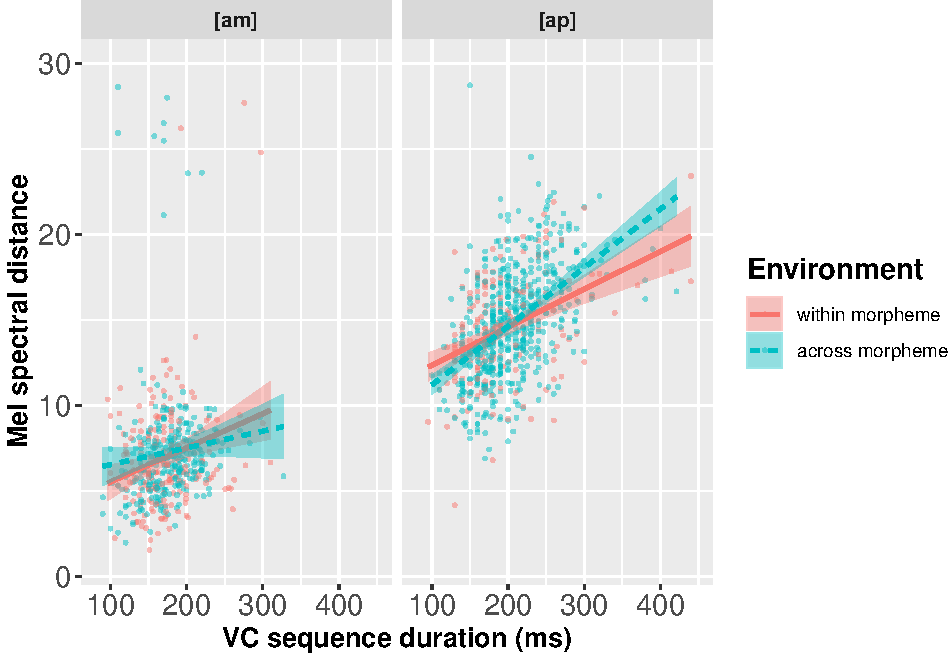
\includegraphics{3_ch3_results_files/figure-latex/adult-int-plot-1.pdf}
\caption{\label{fig:adult-int-plot}Coarticulation within VC sequence by sequence duration and morphological environment in adult speakers}
\end{figure}



Overall, the significance of the interaction \textbf{Sequence duration}, \textbf{VC sequence}, and \textbf{Environment} in adult speakers shows two important results: first, adults distinguish by word environment, both for {[}ap{]} versus {[}a\#p{]} sequences and {[}am{]} versus {[}a\#m{]} sequences. Second, complicating this finding, is the fact that adults distinguish between word environments differently depending upon the VC sequence. For {[}ap{]}, though adults coarticulate roughly equally across and within morphemes, the relationship between duration and coarticulation (longer duration equates to less coarticulation) is stronger in the `across morpheme' condition. For {[}am{]}, adults also distinguish between the two morphological environments by the relationship of VC duration and coarticulatory degree, but the effect of condition is reversed: the relationship between duration and coarticulation is stronger for the `within morpheme' condition.

Thus, returning to one of the central research questions---does adult coarticulation differ by word environment---we find that adults do coarticulate differently in the two word environments. Despite the differences by word environment, there was still a positive relationship between duration and amount of coarticulation for all combinations of VC sequences and word environments. Adults consistently coarticulate less in longer-duration sequences. This result suggests that adult speakers may have one overarching articulatory plan for all environments and both VC sequences measured. The following section demonstrates how this relationship between duration and coarticulation may not be uniform between adults and children.


~

\subsubsection{Children}\label{children}

In the child model, the significant interaction of \textbf{Sequence duration}, \textbf{VC sequence}, and \textbf{Environment} suggests that children do not coarticulate similarly in longer-duration sequences for all combinations of \textbf{Environment} and \textbf{VC sequence} (Figure \ref{fig:child-int-plot}). Specifically, for {[}ap{]} sequences that occur across morpheme boundaries, the negative slope indicates that children actually coarticulate \emph{more} in longer duration sequences. The positive slope for the within morpheme boundary condition suggests that children coarticulate less in longer-duration sequences, in line with all of the adult patterns. So, children coarticulate more between segments at morpheme boundaries in words inflected with the locative marker \emph{-pi} than between those same segments that occur within morphemes.

\begin{figure}[H]
\centering
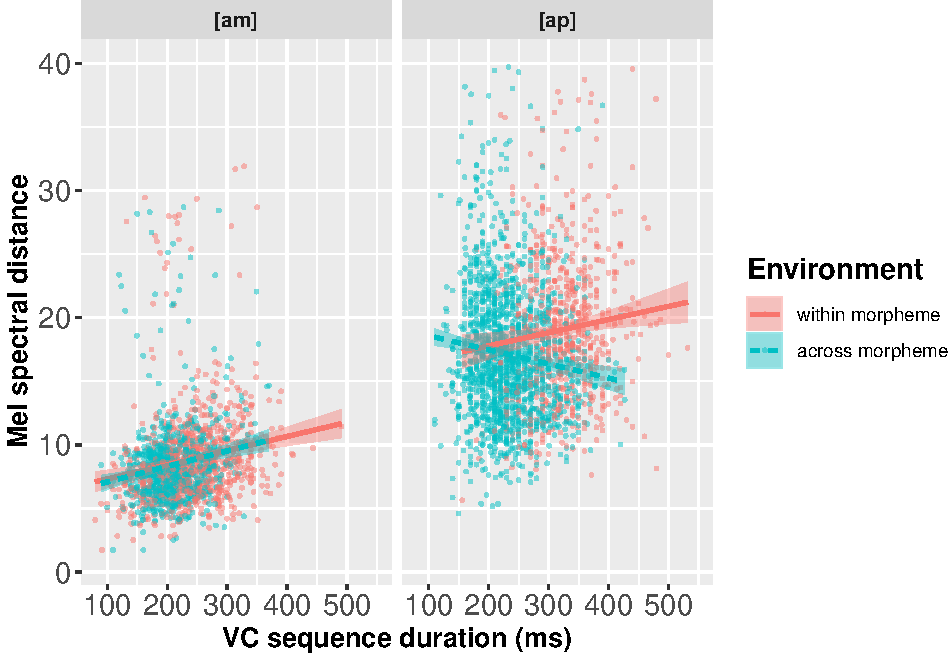
\includegraphics{3_ch3_results_files/figure-latex/child-int-plot-1.pdf}
\caption{\label{fig:child-int-plot}Coarticulation within VC sequence by sequence duration and morphological environment in all child speakers}
\end{figure}

\begin{figure}
\centering
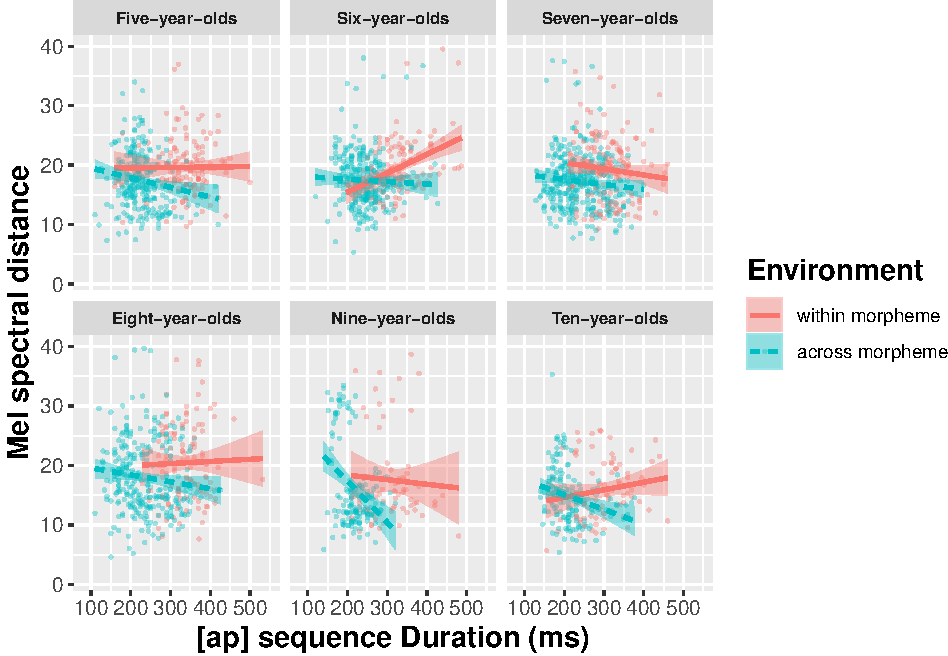
\includegraphics{3_ch3_results_files/figure-latex/child-facet-ap-1.pdf}
\caption{\label{fig:child-facet-ap}Coarticulation within {[}ap{]} by sequence duration, morphological environment, and age in child speakers}
\end{figure}

This negative relationship between duration and spectral distance is counter to the positive relationship for every combination of VC sequence and word environment in adult speakers. Adults consistently coarticulate less in longer-duration sequences regardless of environment or VC sequence. The facet plot in Figure \ref{fig:child-facet-ap} plots this relationship between duration and coarticulation for {[}ap{]} for each age group (5-10 years) to ensure a consistent pattern. All age groups show the same negative relationship: the longer the {[}ap{]} sequence, the more the children coarticulate between {[}a{]} and {[}p{]} in the across morpheme condition.

\begin{figure}
\centering
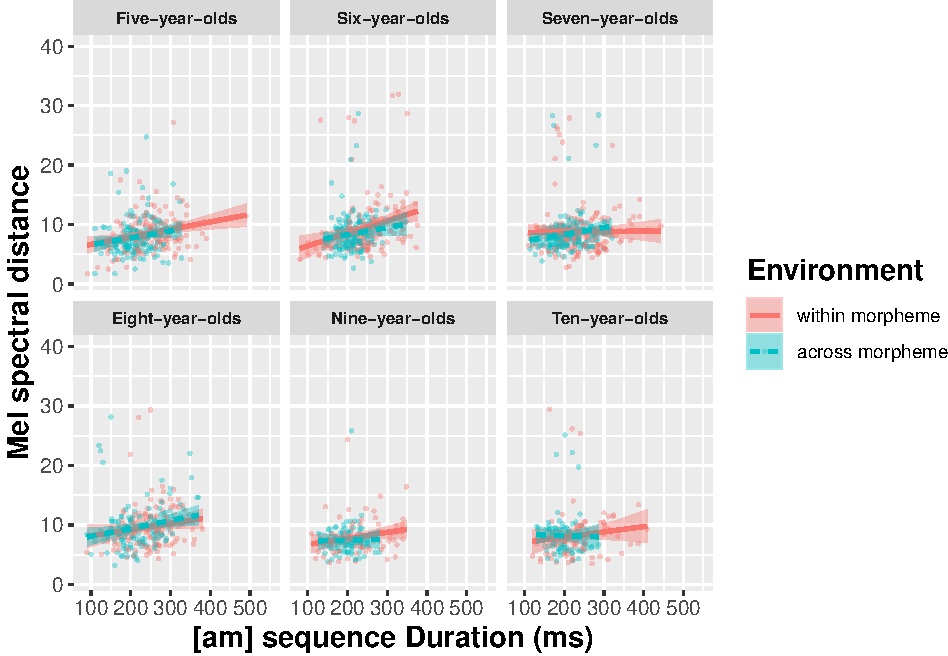
\includegraphics{3_ch3_results_files/figure-latex/child-facet-am-1.pdf}
\caption{\label{fig:child-facet-am}Coarticulation within {[}am{]} by sequence duration, morphological environment, and age in child speakers}
\end{figure}

The results for {[}am{]} in children demonstrate broadly similar results to the adult speakers: children coarticulate less between segments in longer-duration {[}am{]} sequences. The facet plot in Figure \ref{fig:child-facet-am} once again shows a similar effect for each age group. Given the between-subject variability that typically characterizes child speech, these patterns by environment are further broken apart by individual child for each age group (age 5-10) (Appendix I) to ensure no large outliers with regards to the patterning by word environment. The results by are broadly similar across speakers.

In sum, modeling results suggest that morphological structure is reflected in the speech of adults and children. However, the structure manifests in different ways between the two groups. Adults have a single plan for both environments, and even both VC sequences: adults coarticulate less in longer-duration sequences. For the most part, children show a similar duration-coarticulation relationship. The stark difference between adults and children emerges in the {[}ap{]} sequence patterning. Children differentiate between morphological environments via the relationship between duration and coarticulation as they coarticulate more in longer-duration sequences across morpheme boundaries and coarticulate \emph{less} in longer-duration sequences within morphemes. For words inflected with \emph{-man}, children show a similar pattern to adults, though children do not differentiate by environment coarticulatorily. Rather, across morpheme sequences are shorter in duration than within morpheme sequences for the children.


~
~

\subsection{Compensatory shortening}\label{compensatory-shortening}

One finding that emerged from the modeling in the previous section was a different effect of word length on coarticulation between the adults and children. The degree of children's coarticulation tended to progressively increase in words with more syllables; no such pattern was apparent for the adults.

An exploratory analysis was conducted to explain the different relationship between coarticulation and word length for adults and children. This analysis asks, does the direction of the relationship between word length and coarticulation also hold for duration? Since coarticulation and duration are negatively correlated, this analysis predicts that duration would decrease as a function of the number of syllables in a word for children. As such, the children's productions would reflect the phenomenon of \textsc{Compensatory Shortening} (also known as polysyllabic shortening), or the tendency for segment durations to shorten in longer-duration and/or polysyllabic words (\citealt{harringtonRelationshipProsodicWeakening2015}; \citealt{lehistePerceptionCoarticulationEffects1972}; \citealt{munhallCompensatoryShorteningMonosyllables1992}).

An effect of word length upon duration was predicted for the adults as well. However, just as it was found that coarticulation did not increase as a function of word length in the adult model, it is anticipated that adults likewise will not compensate durationally for longer words. As a result, the children, but not the adults, would exhibit compensatory shortening during their word production.

\begin{figure}
\centering
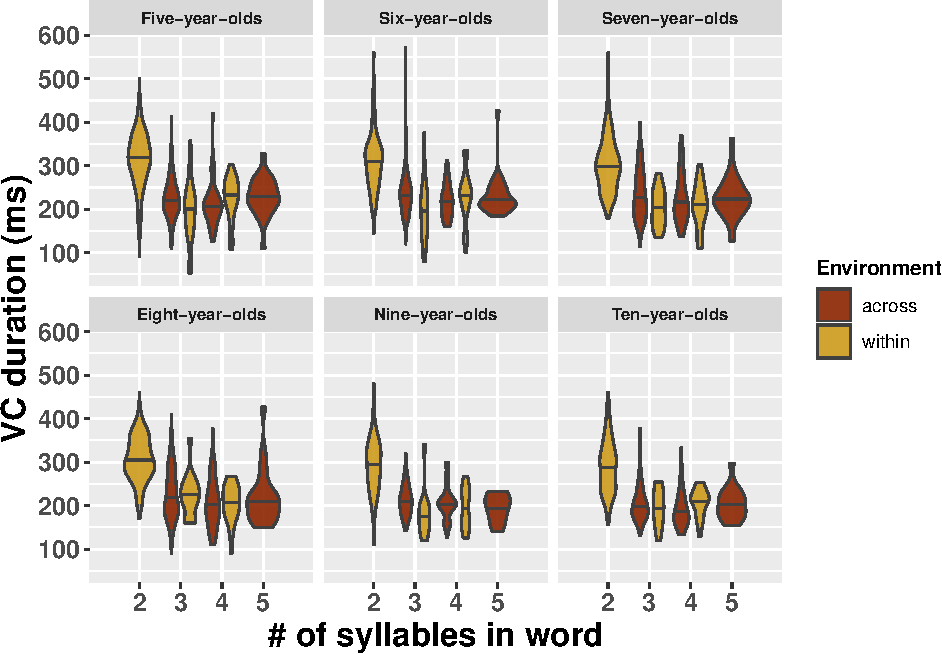
\includegraphics{3_ch3_results_files/figure-latex/compshort-kids-1.pdf}
\caption{\label{fig:compshort-kids}Sequence duration by word length and word environment: Children}
\end{figure}

\begin{figure}
\centering
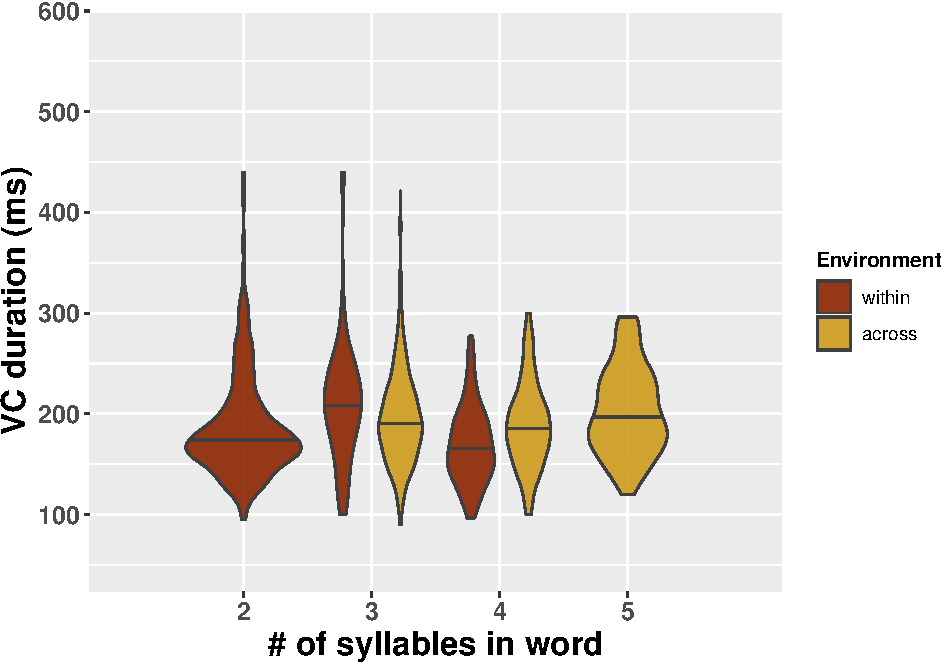
\includegraphics{3_ch3_results_files/figure-latex/compshort-adults-1.pdf}
\caption{\label{fig:compshort-adults}Sequence duration by word length and word environment: Adults}
\end{figure}

\begin{table}[!htbp] \centering 
  \caption{Model predicting VC duration: children} 
  \label{tab:child-dur-model} 
\begin{tabular}{@{\extracolsep{5pt}}lc} 
\\[-1.8ex]\hline 
\hline \\[-1.8ex] 
 Intercept & 230.96$^{***}$ \\ 
  & (228.03, 233.88) \\ 
  & \\ 
 Age:6 & 8.66$^{***}$ \\ 
  & (4.74, 12.58) \\ 
  & \\ 
 Age:7 & 3.78$^{*}$ \\ 
  & (0.43, 7.12) \\ 
  & \\ 
 Age:8 & 0.25 \\ 
  & ($-$4.26, 4.76) \\ 
  & \\ 
 Age:9 & $-$14.46$^{***}$ \\ 
  & ($-$20.31, $-$8.61) \\ 
  & \\ 
 Age:10 & $-$17.23$^{***}$ \\ 
  & ($-$22.92, $-$11.54) \\ 
  & \\ 
 VC sequence:[ap] & 28.31$^{***}$ \\ 
  & (24.38, 32.23) \\ 
  & \\ 
 Two syllables & 57.70$^{***}$ \\ 
  & (54.37, 61.03) \\ 
  & \\ 
 Three syllables & $-$21.63$^{***}$ \\ 
  & ($-$23.54, $-$19.72) \\ 
  & \\ 
 Four syllables & $-$33.27$^{***}$ \\ 
  & ($-$37.97, $-$28.56) \\ 
  & \\ 
\hline \\[-1.8ex] 
Observations & 3,877 \\ 
Log Likelihood & $-$20,476.84 \\ 
Akaike Inf. Crit. & 40,977.68 \\ 
Bayesian Inf. Crit. & 41,052.84 \\ 
\hline 
\hline \\[-1.8ex] 
\textit{Note:}  & \multicolumn{1}{r}{$^{*}$p$<$0.05; $^{**}$p$<$0.01; $^{***}$p$<$0.001} \\ 
\end{tabular} 
\end{table}

\begin{table}[!htbp] \centering 
  \caption{Model predicting VC duration: adults} 
  \label{tab:adult-dur-model} 
\begin{tabular}{@{\extracolsep{5pt}}lc} 
\\[-1.8ex]\hline 
\hline \\[-1.8ex] 
 Intercept & 174.41$^{***}$ \\ 
  & (169.18, 179.63) \\ 
  & \\ 
 VC sequence:[ap] & 29.66$^{***}$ \\ 
  & (22.49, 36.83) \\ 
  & \\ 
 Two syllables & $-$6.12 \\ 
  & ($-$13.46, 1.23) \\ 
  & \\ 
 Three syllables & 4.24$^{*}$ \\ 
  & (0.78, 7.70) \\ 
  & \\ 
 Four syllables & $-$5.36 \\ 
  & ($-$12.97, 2.25) \\ 
  & \\ 
\hline \\[-1.8ex] 
Observations & 1,200 \\ 
Log Likelihood & $-$6,133.52 \\ 
Akaike Inf. Crit. & 12,281.04 \\ 
Bayesian Inf. Crit. & 12,316.67 \\ 
\hline 
\hline \\[-1.8ex] 
\textit{Note:}  & \multicolumn{1}{r}{$^{*}$p$<$0.05; $^{**}$p$<$0.01; $^{***}$p$<$0.001} \\ 
\end{tabular} 
\end{table}

To test the effect of word length (in syllables) upon duration, two linear mixed effects models (adult and child) were fit to predict VC sequence duration (no skewed or non-negative predictors were included in the modeling so GLMMs were not necessary). Model fitting occurred as before in a forward-testing manner: the base model contained random slopes of individual \textbf{Speaker} by \textbf{Word}. Then, parameters were added in the following order: \textbf{Age Group} (fit with weighted effect coding; only included in the child model), \textbf{VC sequence}, \textbf{Number of Syllables} (2-5), and \textbf{Environment} (across versus within). Only the predictors \textbf{Number of Syllables}, \textbf{Age Group}, and \textbf{VC sequence} improved baseline model fit (see Table \ref{tab:child-dur-model} for the child model summary and Table \ref{tab:adult-dur-model} for the adult model summary; see Appendices G and H for tables with descriptive statistics of duration by age and number of syllables).

In both model summaries, the positive beta coefficients for VC sequence indicate that the {[}ap{]} sequence was significantly longer than the {[}am{]} sequence (as previous models demonstrated). The insignificance of \textbf{Environment} suggests that that the relationship between duration and word length is independent of word environment. The patterns by child age again demonstrate how older children speak faster than younger. Negative coefficients for the nine- and ten-year old children indicate that those children's VC sequences were approximately 14 ms and 17 ms shorter, respectively, than the weighted age group mean.

The primary parameter of interest is \textbf{Syllable Count}. In the child model, the positive coefficient for `2 syllable' stimuli indicates that VC sequence duration in two syllable words was approximately 58 ms longer than the weighted mean word length. The negative coefficients for the `3 syllable' (\(\beta\)=-21.63), `4 syllable' (\(\beta\)=-33.27) and `5 syllable' (\(\beta\)=-28.62; not presented in model summary) stimuli indicate that VC sequences tend to become shorter in longer words. The diverse stimuli in the two- and three-syllable conditions in particular (many different word types) suggest that this relationship by word length is relatively robust for the children.\footnote{The only exception to the tendency to shorten sequences in larger words was that {[}ap{]} sequences are slightly longer in duration in 5-syllable words than 4-syllable words. However, in this exploratory analysis, the differences between the four and five syllable words were not tightly controlled: there were only two different five-syllable word stimuli: \emph{hatun mama-man} `grandmother-\textsc{all}'' and \emph{hatun mama-pi} `grandmother-\textsc{loc}'. We can only speculate that this relationship between sequence duration and number of syllables is strictly linear and would generalize to additional words with more syllables for the children.}

For the adult model, \textbf{Syllable Count} only marginally improved over one without (\(\chi\)\textsuperscript{2} = 6.72, df=4,7, p=.08). Furthermore, only one level of \textbf{Syllable Count}, the three syllable stimuli, significantly predicted sequence duration. This result suggests that 1) word length was not strongly predictive of sequence duration in the adults and 2) adults did not compensate for word length by shortening syllable durations in longer words.

In sum, children appear to compensate for word length in their speech production via coarticulation and duration. Word length is also reflected in the adults' speech patterns, but not in any linear direction that suggests compensatory shortening. Causes behind these age differences are proposed in the Discussion.






~
~

\section{Discussion}

This study measured the acoustic patterns of adult and child Quechua speakers within and across morpheme boundaries. Two predictions were made: 1) adult speakers would coarticulate less between two phones at a morpheme boundary than between the same phones within a morpheme boundary, and 2) child speakers would coarticulate more than adults between phones at morpheme boundaries. The reasoning behind these hypotheses was that frequency ratios between suffixes, and between roots and suffixes, predict decompostability in adults (\citealt{hayCausesConsequencesWord2003}; \citealt{kempsProsodicCuesMorphological2005}; \citealt{ingoplagSuffixOrderingMorphological2009}). Adult speakers have more experience with language than children, and have larger vocabularies \citep{lorgeEstimatingSizeVocabularies1963}. Consequently, adults may weigh the ratios of inflected to base forms in their lexicons differently. And children may structure relationships between base and suffixal forms differently as they age and their vocabularies grow. For these reasons, it was predicted that the adults' patterns by environment may differ from the children's. 

Results confirmed that adult speakers differentiated by word environment in their speech, but so did the children. However, the two groups differentiated by environment in distinct ways. Adults reliably coarticulated more in shorter-duration sequences in all combinations of VC sequence and word environment suggesting that they have one, overarching articulatory plan for these VC sequences. Differentiation by morphological environment in adult speech hinged on the strength (i.e., the slope) of the relationship between duration and coarticulation. Children instead differentiated by environment via duration ([am] sequences) or the relationship between coarticulation and duration ([ap] sequences). Thus, the children's patterns were simultaneously distinct from and similar to the adults'. 

\subsection{How is morphological structure reflected in participants' speech production?}

Adults distinguished between the word environments in their speech production, though they did not necessarily coarticulate more within morphemes than across. Instead, adults used a combination of duration and coarticulation as they consistently coarticulated more in shorter-duration sequences. This reflection of morphological structure in the adult speakers' speech might be expected if, as previous studies suggest, speech production---coarticulation and duration in the current study---indexes lexical retrieval and composition (\citealt{choEffectsMorphemeBoundaries2001}; \citealt{kempsProsodicCuesMorphological2005}; \citealt{lee-kimMorphologicalEffectsDarkness2013}; \citealt{plagHomophonyMorphologyAcoustics2017}; \citealt{pluymaekersMorphologicalEffectsFine2010}; \citealt{songEffectsCoarticulationMorphological2013}; \citeyear{songDurationalCuesFricative2013}; \citealt{sugaharaDurationalCorrelatesEnglish2009}; \citeauthor{tomaschekHowAnticipatoryCoarticulation2019} \textit{under review}). The adult speakers may differentiate between word environments because they compose morphologically complex words from their component parts. Though decomposition is probabilistic (e.g., \citealt{hayCausesConsequencesWord2003}), overall, the speech production data do not suggest that adults are accessing morphologically complex words holistically. 

Child speakers of all ages (5-10 years) also differentiated by word environment in their speech, suggesting that they may be composing the complex words online. The data suggest that this does not change over development and that children as young as five appear to have awareness of morphological boundaries. However, the children's patterns by word environment differed from the adults'. In slower speech, adult speakers coarticulated less, both across and within morphemes, replicating known interactions between speaking rate (here instantiated as VC sequence duration) and coarticulation (\citealt{agwueleEffectSpeakingRate2008}; \citealt{gayMechanismsControlSpeech1981}; \citealt{matthiesVariationAnticipatoryCoarticulation2001}). In children, the same relationship between VC sequence duration and coarticulation appeared in the within-morpheme condition where children coarticulated less when they spoke slower. However, unexpectedly, the children coarticulated \textit{more} in longer duration [ap] sequences.

The similarities between adults and children concerning the coarticulation-duration relationship are expected since 1) speakers coarticulate more in faster speech and 2) there is no a priori reason to assume that the direction of the relationship between coarticulation and duration should differ in children, even if they coarticulate more or less overall than adults (see Section \ref{child-coartic}). The children in this study spoke slower than the adults: the average VC sequence duration for the adults was just 192 ms ($\sigma$=47) compared to 252 ms ($\sigma$=69) for the five-year-olds, 255 ms ($\sigma$=70), for the eight-year-olds, and 231 ms ($\sigma$=63) for the ten-year-olds. Yet the fact that even the youngest children demonstrated this expected coarticulation-duration relationship in most of their data (with the exception of [ap] between morphemes) suggests the direction of the relationship between the two speech measures is consistent across different speech speeds. Children also seem to acquire it by age 5, if not sooner. 

The unexpected pattern for [ap] between morphemes warrants exploration. Why did children coarticulate more in longer-duration [ap] sequences? The effect is robust across all word types in the condition (Appendix F), and all child age groups (Figure \ref{fig:child-facet-ap}), suggesting that neither word frequency nor language experience \textit{within} the children explain the pattern. In other words, because the effect occurs for all child age groups, it seems unlikely that it reflects lexical organization or access. The ratios between suffixes and roots re-organize between ages 5 and 10 as children's vocabularies grow, yet the coarticulation-duration relationship is consistent across child age groups. So there must be one or more overarching differences between the adults and children, besides age and its accompanying lexical reorganization, that could explain the [ap] pattern. Section \ref{adult-child-diff} proposes one such explanation---adults' greater dominance in Quechua---that may explain these age differences. This explanation could likewise explain why children compensate for word length in their speech production but adults do not. Consequently, the following section first discusses the findings about word length effects on speech production. 

\subsection{Compensatory shortening}\label{comp-lengthen}

One additional difference between the adults and children was that children compensated for word length by shortening the duration of their VC sequences in longer words (or, variably, lengthening duration in the shorter words). This phenomenon is known as compensatory shortening (\citealt{harringtonRelationshipProsodicWeakening2015}; \citealt{lehisteTimingUtterancesLinguistic1972}; \citealt{munhallCompensatoryShorteningMonosyllables1992}).\footnote{The term compensatory shortening is also variably used in the literature to refer to shortening of stressed vowels compared to unstressed vowels in the context of polysyllabicity \citep{harringtonRelationshipProsodicWeakening2015}, or the shortening of stressed vowels in the context of unstressed vowels and consonants \citep{fowlerRelationshipCoarticulationCompensatory1981}.}  While children demonstrated a trade-off in sequence duration and prosodic word size, adults were insensitive to word size. As described in the literature review, the children's compensatory shortening reinforces previous work, conducted on adult speech, that has demonstrated how roots can have different variants in their bound and free forms \citep{kempsProsodicCuesMorphological2005}. This is because the prosodically-longer stimuli were often bound forms of free roots (e.g., bound root \textit{llama-pi} `llama-\textsc{loc}' and free root \textit{llama} `llama'). One challenge in the study of morphophonetics has been to identify the explanatory mechanisms behind morphologically-conditioned speech variation; at least in the child data, compensatory shortening could be one of these mechanisms. 

This relationship between word size and segment duration in the children's speech is notable. The data indicate that the children could have some minimal planning unit size causing them to elongate prosodically short words (or shorten prosodically long words) to fit within the unit's temporal domain. However, possibly even more interesting than the children's patterns is the \textit{lack} of compensatory shortening in the adults because previous findings on compensatory shortening came from adult populations. Why don't adults in the current study compensate for word size in their speech production as the children, even the eldest ten-year-olds, appear to?

\subsection{Explaining differences between adults and children}\label{adult-child-diff}

Two differences between adult and child speech patterns have emerged in the Discussion: 1) children, but not adults, coarticulate more in longer-duration, across-morpheme [ap] sequences and 2) children, but not adults, compensate temporally for word length. One explanation for the compensatory shortening difference by age is that adults speak faster than children \citep{leeAcousticsChildrenSpeech1999}, leading to more extreme phonetic reduction in adult speech. Children do not approximate adult-like speaking rates until early puberty (\citealt{leeAcousticsChildrenSpeech1999}; \citealt{smithRelationshipsDurationTemporal1992}). And this increase in speaking rate by age is replicated in the present study (see Tables \ref{tab:ap-dur-tbl} and \ref{tab:am-dur-tbl} in the Results). Speaking rate is relevant for compensatory shortening because adult Quechua speakers may speak so much faster, and reduce so much more, than children that there could be insufficient freedom in their speech duration to differentiate sequence duration by prosodic word size. Speakers reduce significantly more in fast speech compared to slower, controlled speech. In fast speech, the vowel space is smaller and more centralized (\citealt{fourakisTempoStressVowel1991}; \citealt{tsaoEffectIntertalkerSpeech2006})---which may compromise contrasts \citep{koopmans-vanbeinumVowelContrastReduction1980}, increase coarticulation between phones (\citealt{agwueleEffectSpeakingRate2008}; \citealt{matthiesVariationAnticipatoryCoarticulation2001}), and cause the omission of entire segments or syllables \citep{johnsonMassiveReductionConversational2004}. For the current study, the durational data by age suggest that all adult speech, regardless of prosodic or morphological structure, is maximally fast and reduced.  

Though there is little work on the phonetics of highly morphologically complex languages, the author can anecdotally attest to how speaking rate interplays with word structure in Quechua. Just as the orthographic forms of English words rarely correspond to their phonetic realization in fast, spontaneous speech, spoken words in Quechua deviate from their citation form. In Quechua, this is especially true with large words that contain numerous suffixes, where the most extreme reduction can be seen. In Quechua, the further a suffix is found from the root, the \textit{more} likely it is to be reduced (shorter in duration, omission of segments and/or syllables). The explanation for this is partially aerodynamic (e.g., airflow). But there are also likely perceptual and information-theoretic explanations. When suffixes are highly reduced compared to stems, speakers can more easily demarcate between suffixes and roots, and identify word boundaries \citep{zinglerReductionFusionGrammaticalization2018}. Furthermore, word meanings are likely increasingly predictable as additional suffixes are added and the available semantic space of the word narrows.\footnote{For English, however, Plag and Baayen (2009) found that those suffixes farthest from the stem are also the most productive and available for use in novel environments.} Variability in the phonetic realization of English morphology (e.g., plurals) is dependent upon the predictability of plurality given the sentence frame \citep{cohenProbabilisticReductionProbabilistic2014}, so it is possible that speakers likewise make probability calculations over multiple suffixes. Much more work is needed to understand probabilistic reduction based on word structure. However, overall, one explanation for adults' lack of compensatory lengthening is their speaking rate and phonetic reduction.

A second explanation for the lack of compensatory shortening in adults, that may also explain the unexpected coarticulation-duration relationship in children's [ap] sequences, is that the adults are more dominant in Quechua than the children. First, this means that the adults may speak faster and, again, may be unable to temporally differentiate prosodic structures. It also means that the adults are more likely to have uniform, established articulatory speech plans in Quechua because they use the language more. For example, the adults studied here reliably coarticulate more in faster speech. It would not be surprising if the children, who have less Quechua experience, had not yet established reliable speech plans for all word environments and phone sequences in Quechua.

Recent changes in Bolivia's educational policy, as well as the country's general sociolinguistic situation, may have led to adults' increased Quechua dominance. Bilingual education in Bolivia became mandatory in 1994 and has, in theory, been relatively widespread since the early 2000s \citep{bensonBilingualSchoolingMozambique2004}. This means more children, especially indigenous students and young girls, are attending and completing more schooling than ever before \citep{hornbergerMultilingualEducationPolicy2009}. 

In practice, however, bilingual education often takes the form of Spanish-only classrooms. In Quechua-speaking areas, many trained teachers do not speak Quechua fluently or are not provided with teaching materials and textbooks written in Quechua. The result---students completing more schooling but instructed in Spanish---has been rapid language shift \citep{hornbergerLanguageRevitalisationAndes1996}. This has been apparent even within the last decade, as the first generation of women educated in this system are now raising their children using both Quechua and Spanish, instead of monolingual Quechua, in an increasingly Spanish-dominant environment. 

These sociolinguistic dynamics could manifest in the present sample as the adult female participants (many of whom are mothers) may be more Quechua-dominant than some of the children in the sample. Though the adult females who participated in the study were only, on average, 13 years older than the eldest children (adult $\mu$\textsubscript{age}=23 years; $\sigma$=5.46 years), and all adults and children identified as bilingual Quechua-Spanish speakers, their language practices may reflect the recent changes in educational policy. It is also important to note that all of the children in the sample attended school, in Spanish, for 3-4 hours per day. However, only one of the adult females was still attending school (taught in Spanish). This difference could also explain usage patterns between the age groups.

If the adult females were more Quechua-dominant, or used Quechua more frequently, they would speak faster, more fluently, and could reduce more, with ramifications for speech production described above. The adults would also have established, uniform articulatory strategies, such as consistently coarticulating more in faster speech, for all segments, in all word environments. Thus, although the adult speakers in this study undoubtedly did speak faster than the children for speech maturation reasons---it takes time and practice to master the articulatory speed of an adult \citep{leeAcousticsChildrenSpeech1999}---the adults may also have spoken Quechua faster, and thus failed to compensate for prosodic structure to the degree that the children did, because they use Quechua more frequently. This proposal may not entirely explain the differences between the adult and child Quechua speakers. For one thing, previous studies on compensatory shortening (\citealt{lehisteTimingUtterancesLinguistic1972}; \citealt{munhallCompensatoryShorteningMonosyllables1992}) reported on highly-fluent, monolingual adult speakers who \textit{did} compensate for prosodic structure. Also, if increased language experience with Quechua predicts uniform articulatory strategies, then we might anticipate that ten-year-olds would have more uniform strategies than five-year-olds. However, these clear differences in language usage and experience between adults and children, independent of age, may explain some of the speech production differences observed between the groups. 

\subsection{Effects of bilingual status}

Given that all of the participants in this study were bilingual, it is important to note the potential role of Spanish language use and contact upon the results. First, although participants were not literate in Quechua, most were literate (or becoming literate given the age range) in Spanish. Nevertheless, it is unlikely that Spanish literacy would translate to increased awareness of morphological structure in Quechua. Spanish and Quechua's distinct morphological typologies make this transfer of awareness unlikely. Quechua is more synthetic than Spanish (words tend to carry more unique morphemes). Spanish is also highly fusional while Quechua is strictly agglutinating---each morpheme carries a unique grammatical role. The typological distance between the languages is unlikely to facilitate much crossover awareness of word structure (prosodic or morphological). 

Beyond literacy, the children's bilingual Quechua-Spanish status could have influenced the results if it increased between-subject variability. This study did not report participants' bilingual language dominance, but all speakers identified as Quechua-Spanish bilinguals and reported using both languages. However, bilingual children, including those in the current study, are rarely exposed to or use equal quantities of their two languages \citep{orenaWhatBilingualInfants2020}. Naturalistic assessments of the child Quechua-Spanish speakers' bilingual language practices has been reported elsewhere \citep{cychoszPhoneticDevelopmentAgglutinating2020}; results showed that there is variability in the amount of Spanish and Quechua that the children use.\footnote{ The decision not to conduct a traditional language usage survey was made for several reasons. Traditional measures of self-reported bilingual dominance, such as the bilingual language profile \citep{birdsonBilingualLanguageProfile2012}, often rely on participant literacy or familiarity and comfort with written behavioral research surveys. Also, the traditional stigmatization of indigenous languages in Bolivia may render self-reports of language dominance unreliable.} These individual differences even explained some variability in the children's coarticulation patterns. Consequently, one difference between speakers that was not explored in this study is bilingual Quechua-Spanish language use.\footnote{It is important to note that all children in Bolivia acquire Spanish in school making a more controlled sample of monolingual school-aged children difficult to find.}  

\subsection{Future work}

Future work, ideally on languages with different and complex word structures, is needed to further explore the relationships between children's speech production and word structure. Going forward, researchers may also benefit from the use of articulatory measures, in addition to acoustic, to explore the relationships between coarticulation and morphological structure in children. Given the logistics of ultrasound imaging, and the limitations of fieldwork, the current study was not able to collect articulatory data, which would otherwise be a valuable addition.

This study was also unable to control for, or examine the effect of, lexical frequency of the base or inflected forms. Instead, a greater number of diverse word types were included to mitigate any potential extreme lexical frequency effects. The absence of frequency statistics is unfortunate because much variability in morphological parsing, and morphophonetics, is attributable to lexical frequency \citep{seyfarthAcousticDifferencesMorphologicallydistinct2018} or frequency ratios between stems and suffixes (\citealt{hayCausesConsequencesWord2003}; \citealt{ingoplagSuffixOrderingMorphological2009}). At this time, however, it is not possible to reliably calculate these statistics for Quechua, and indeed for most of the world's languages. The author recently collected a large, naturalistic corpus of child and adult Bolivian Quechua, but it will be years before it is sufficiently transcribed to calculate lexical statistics. In the mean time, researchers interested in the morphophonetics of underdocumented languages could possibly use age of acquisition as a proxy for word frequency \citep{morrisonAgeAcquisitionNot1992} and this may a promising methodological approach should researchers hope to include additional under-documented languages in the study of morphophonetics.\footnote{The author found that obtaining age of acquisition norms was not possible for the current study because the Quechua-speaking adults were relatively unfamiliar with behavioral research and the methods that would have been required to solicit age of acquisition information.} 


\section{Conclusion}

This study measured adult and child Quechua speakers' speech patterns in two morphological environments: within morphemes and across morpheme boundaries. Using a combination of coarticulatory and temporal cues, adults and children distinguished between the two morphological environments in their speech production, though they did so in distinct ways. This replicated known speech production patterns by word environment but in an understudied, morphologically complex language. The children also showed increased prosodic sensitivity where the adults did not: children shortened the duration of sequences in prosodically longer words. It was suggested that the difference between adults and children could be attributable to adults' faster speaking rate and increased practice with Quechua. Overall, these analyses have demonstrated the complex ways that morphological structure can be reflected in speech and how those patterns change with language experience. Overall, this study has demonstrated the importance of extending recent studies on morphophonetics to languages with vastly different word structures and speakers with different language backgrounds. 

\section*{Declaration of interest}
The author has no competing interests to report. 

\section*{Acknowledgements}


\theendnotes

\bibliography{zotero_library}

\appendix
\section{South Bolivian Quechua Consonant Inventory}\label{app:app-A}

\begin{table}

\centering
	\begin{tabular}{l|c|c|c|c|c|c|c|c|c|c}
			    & 
				\multicolumn{1}{c|}{\footnotesize{Bilabial}} &					% Bilabial
				\multicolumn{1}{c|}{\footnotesize{Dental}} & 					% Dental
				\multicolumn{1}{c|}{\footnotesize{Postalveolar}} & 		% Post-alveolar
		       \multicolumn{1}{c|}{\footnotesize{Palatal}} & 		
		       % palatal
				\multicolumn{1}{c|}{\footnotesize{Velar}} & 					% Velar
				\multicolumn{1}{c|}{\footnotesize{Uvular}} & 					% Uvular
				\multicolumn{1}{c}{\footnotesize{Glottal}}  \\					% Glottal

			\hline Plosive &  % Plosive
			        \textipa{p}  & % bilabial
			        \textipa{t}	&	% Dental
					\textipa{\textteshlig}	& % Post-alveolar
					\Blankcell &	% Palatal
				    \textipa{k} &	% Velar
			      	\textipa{q} &	% Uvular
				   \Blankcell \\	% Glottal
				   
		     \hline Aspirated &  % Plosive
			        \textipa{p}\textsuperscript{h}  & % bilabial
			        \textipa{t}\textsuperscript{h}	&	% Dental
					\textipa{\textteshlig}\textsuperscript{h}	& % Post-alveolar
					\Blankcell &	% Palatal
				    \textipa{k}\textsuperscript{h} &	% Velar
			      	\textipa{q}\textsuperscript{h} &	% Uvular
				   \Blankcell \\	% Glottal
				   
			 \hline Ejective &  % Plosive
			        \textipa{p}'  & % bilabial
			        \textipa{t}'	&	% Dental
					\textipa{\textteshlig}'	& % Post-alveolar
					\Blankcell &	% Palatal
				    \textipa{k}' &	% Velar
			      	\textipa{q}' &	% Uvular
				   \Blankcell \\	% Glottal

			\hline Nasal & 	% Nasal
				\textipa{m} & % Bilabial
				\textipa{n}	& % Dental
			    \Blankcell & % Post-alveolar
			    \textltailn &	% Palatal
				\Blankcell  & % Velar
				\Blankcell	& % Uvular
				\Blankcell \\% Glottal

			\hline Fricative &  % Fricative
				\Blankcell &	% Labial
				\ipa{s} & % Dental
			    \Blankcell	& % Post-alveolar
			    \Blankcell &	% Palatal
				\Blankcell	& % Velar
				\Blankcell	& % Uvular
				\textipa{h}	\\ % Glottal
				
			\hline Tap & % Tap 
				\Blankcell	& % Bilabial
				\textfishhookr & % Dental
				\Blankcell	& % Post-alveolar
				\Blankcell &	% Palatal
				\BlankCell 	& % Velar
				\Blankcell	& % Uvular
				\BlankCell  \\ % Glottal

			\hline Approximant & % Approx.
				\textipa{w} & % Bilabial
				\BlankCell	& % Dental
				\textturny 	& % Post-alveolar
				\textipa{j} &	% Palatal
				\Blankcell & % Velar
				\Blankcell & % Uvular
				\BlankCell \\ % Glottal

			\hline Lateral & % Lateral
				  \BlankCell  & % Bilabial
			      \textipa{l} & % Dental
				  \Blankcell  & % Post-alveolar
				  \Blankcell &	% Palatal
				 \BlankCell &	% Velar
				 \BlankCell  & % Uvular
				 \BlankCell	\\ % Glottal
		\end{tabular}
		\end{table}
		



\section{Stimuli used in real word repetition tasks}\label{app:app-B}
\begin{table}

\centering
\begin{tabular}{c | c} 
\hline
Real word* & Translation  \\
\hline

\footnotesize{\textsf{'}warmi} & `woman' \textit{training trial}\\
\footnotesize{\textsf{'}wasi} & `house' \textit{training trial} \\
\footnotesize{\textsf{'}qhari} & `man' \textit{training trial}\\
\footnotesize{\textsf{'}chita} & `sheep' \\
\footnotesize{\textsf{'}p'esqo} & `bird' \\
\footnotesize{ju\textsf{'}k'ucha} & `mouse' \\
\footnotesize{\textsf{'}waka} & `cow' \\
\footnotesize{\textsf{'}wallpa} & `chicken' \\
\footnotesize{\textsf{'}mama} & `mom' \\
\footnotesize{\textsf{'}papa} & `potato' \\
\footnotesize{\textsf{'}t'ika} & `flower' \\
\footnotesize{\textsf{'}llama} & `llama' \\
\footnotesize{\textsf{'}cuca} & `coca (leaves)' \\
\footnotesize{u\textsf{'}hut'a} & `sandal' \\
\footnotesize{ham\textsf{'}piri} & `healer' \\
\footnotesize{i\textsf{'}milla} & `girl' \\
\footnotesize{\textsf{'}llapa} & `lightning' \\
\footnotesize{\textsf{'}api} & `corn/citrus drink' \\
\footnotesize{\textsf{'}ch'ulu} & `hat' \\
\footnotesize{\textsf{'}punku} & `door' \\
\footnotesize{\textsf{'}thapa} & `nest' \\
\footnotesize{\textsf{'}punchu} & `poncho' \\
\footnotesize{\textsf{'}pampa} & `prairie' \\
\footnotesize{\textsf{'}sunkha} & `beard' \\
\footnotesize{hatun\textsf{'}mama} & `grandma' \\
\footnotesize{\textsf{'}wawa} & `baby/child' \\
\footnotesize{\textsf{'}runtu} & `egg' \\
\footnotesize{\textsf{'}qolqe} & `money' \\
\footnotesize{\textsf{'}q'apa} & `palm of hand' \\
\footnotesize{\textsf{'}alqo} & `dog' \\
\footnotesize{\textsf{'}q'epi} & `bundle' \\
 \hline

\end{tabular}\par
\smallskip
* For the real words, \textsf{'} indicates stress, ' indicates ejective
\end{table}

		
		
\section{Real word repetition stimuli to elicit [ap]}\label{app:app-ap}

\begin{table}
\centering
\begin{tabular}{c | c| c} 
\hline
Real word* & Translation & \thead{Morpheme environment\textsuperscript{\textdagger}}\\
\hline

\footnotesize{chi\textsf{'}t\textbf{a-p}i} & `sheep-\textsc{loc}' & across \\
\footnotesize{cu\textsf{'}c\textbf{a-p}i} & `coca (leaves)-\textsc{loc}' & across \\
\footnotesize{hatunma\textsf{'}m\textbf{a-p}i} & `grandma-\textsc{loc}' & across \\
\footnotesize{imi\textsf{'}ll\textbf{a-p}i} & `girl-\textsc{loc}' & across \\
\footnotesize{juk'u\textsf{'}ch\textbf{a-p}i} & `mouse-\textsc{loc}' & across \\
\footnotesize{lla\textsf{'}m\textbf{a-p}i} & `llama-\textsc{loc}' & across \\
\footnotesize{lla\textsf{'}p\textbf{a-p}i} & `lightning-\textsc{loc}' & across \\
\footnotesize{ma\textsf{'}m\textbf{a-p}i} & `mom-\textsc{loc}' & across \\
\footnotesize{pam\textsf{'}p\textbf{a-p}i} & `prairie-\textsc{loc}' & across \\
\footnotesize{pa\textsf{'}p\textbf{a-p}i} & `potato-\textsc{loc}' & across \\
\footnotesize{q'a\textsf{'}p\textbf{a-p}i} & `palm of hand-\textsc{loc}' & across \\
\footnotesize{sun\textsf{'}kh\textbf{a-p}i} & `beard-\textsc{loc}' & across \\
\footnotesize{t'i\textsf{'}k\textbf{a-p}i} & `flower-\textsc{loc}' & across \\
\footnotesize{tha\textsf{'}p\textbf{a-p}i} & `nest-\textsc{loc}' & across \\
\footnotesize{uhu\textsf{'}t'\textbf{a-p}i} & `sandal-\textsc{loc}' & across \\
\footnotesize{wa\textsf{'}k\textbf{a-p}i} & `cow-\textsc{loc}' & across \\
\footnotesize{wall\textsf{'}p\textbf{a-p}i} & `chicken-\textsc{loc}' & across \\
\footnotesize{wa\textsf{'}w\textbf{a-p}i} & `baby/child-\textsc{loc}' & across \\

\hline

\footnotesize{\textsf{'}p\textbf{ap}a} & `potato' & within \\
\footnotesize{\textsf{'}ll\textbf{ap}a} & `lightning' & within \\
\footnotesize{\textsf{'}\textbf{ap}i} & `corn/citrus drink' & within \\
\footnotesize{\textsf{'}th\textbf{ap}a} & `nest' & within \\
\footnotesize{\textsf{'}q'\textbf{ap}a} & `palm of hand' & within \\

 \hline
\end{tabular}\par
\smallskip
* ' indicates stress, \textsf{'} indicates ejective\par
\end{table}


\section{Real word repetition stimuli to elicit [am]}\label{app:app-C}

\begin{table}\small

\centering
\begin{tabular}{c | c| c} 
\hline
Real word* & Translation & \thead{Morpheme environment\textsuperscript{\textdagger}}\\
\hline

\footnotesize{chi\textsf{'}t\textbf{a-m}an} & `sheep-\textsc{all}' & across \\
\footnotesize{cu\textsf{'}c\textbf{a-m}an} & `coca (leaves)-\textsc{all}' & across \\
\footnotesize{hatunma\textsf{'}m\textbf{a-m}an} & `grandma-\textsc{all}' & across \\
\footnotesize{imi\textsf{'}ll\textbf{a-m}an} & `girl-\textsc{all}' & across \\
\footnotesize{juk'u\textsf{'}ch\textbf{a-m}an} & `mouse-\textsc{all}' & across \\
\footnotesize{lla\textsf{'}m\textbf{a-m}an} & `llama-\textsc{all}' & across \\
\footnotesize{lla\textsf{'}p\textbf{a-m}an} & `lightning-\textsc{all}' & across \\
\footnotesize{ma\textsf{'}m\textbf{a-m}an} & `mom-\textsc{all}' & across \\
\footnotesize{pam\textsf{'}p\textbf{a-m}an} & `prairie-\textsc{all}' & across \\
\footnotesize{pa\textsf{'}p\textbf{a-m}an} & `potato-\textsc{all}' & across \\
\footnotesize{q'a\textsf{'}p\textbf{a-m}an} & `palm of hand-\textsc{all}' & across \\
\footnotesize{sun\textsf{'}kh\textbf{a-m}an} & `beard-\textsc{all}' & across \\
\footnotesize{t'i\textsf{'}k\textbf{a-m}an} & `flower-\textsc{all}' & across \\
\footnotesize{tha\textsf{'}p\textbf{a-m}an} & `nest-\textsc{all}' & across \\
\footnotesize{wa\textsf{'}k\textbf{a-m}an} & `cow-\textsc{all}' & across \\
\footnotesize{wall\textsf{'}p\textbf{a-m}an} & `chicken-\textsc{all}' & across \\
\footnotesize{wa\textsf{'}w\textbf{a-m}an} & `baby/child-\textsc{all}' & across \\

\hline

\footnotesize{\textsf{'}m\textbf{am}a} & `mom' & within \\
\footnotesize{\textsf{'}ll\textbf{am}a} & `llama' & within \\
\footnotesize{h\textbf{am}\textsf{'}piri} & `healer' & within \\
\footnotesize{h\textbf{am}pi\textsf{'}ri-pi} & `healer-\textsc{loc}' & within \\
\footnotesize{\textsf{'}p\textbf{am}pa} & `prairie' & within \\
\footnotesize{hatun\textsf{'}m\textbf{am}a} & `grandma' & within \\

 \hline
\end{tabular}\par
\smallskip
* ' indicates stress, \textsf{'} indicates ejective\par
\smallskip
\end{table}

\section{Model predicting coarticulation in children and adults}\label{app:app-E}

\begin{table}
\begin{center}
\begin{threeparttable}
\resizebox{\columnwidth}{!}{%
\begin{tabular}{llllll}
\toprule
term & \multicolumn{1}{c}{estimate} & \multicolumn{1}{c}{S.E.} & \multicolumn{1}{c}{z.statistic} & \multicolumn{1}{c}{p.value} & \multicolumn{1}{c}{95\% CI}\\
\midrule
Intercept & 204.61 & 4.67 & 43.86 & 0.00 & 2.14,1.95\\
Syllable count:2 & 9.48 & 2.05 & 4.62 & 0.00 & 0.13,0.05\\
Syllable count:3 & -3.31 & 0.95 & -3.47 & 0.00 & -0.01,-0.05\\
Syllable count:4 & -1.12 & 1.36 & -0.82 & 0.41 & 0.02,-0.04\\
Sequence duration & 0.29 & 0.06 & 4.99 & 0.00 & 0,0\\
VC sequence:ap & 61.68 & 5.31 & 11.62 & 0.00 & 0.72,0.51\\
Age:child & 6.07 & 4.75 & 1.28 & 0.20 & 0.15,-0.03\\
Environment:across morpheme & 5.73 & 6.35 & 0.90 & 0.37 & 0.18,-0.07\\
Sequence duration*VC sequence:ap & -0.15 & 0.07 & -2.18 & 0.03 & 0,0\\
Sequence duration*Age:child & -0.21 & 0.06 & -3.39 & 0.00 & 0,0\\
VC sequence:ap*Age:child & 6.83 & 6.10 & 1.12 & 0.26 & 0.19,-0.05\\
Sequence duration*Environment:across morpheme & -0.11 & 0.08 & -1.31 & 0.19 & 0,0\\
VC sequence:ap*Environment:across morpheme & 9.12 & 6.95 & 1.31 & 0.19 & 0.23,-0.05\\
Age:child:Environmentacross morpheme & 0.42 & 6.30 & 0.07 & 0.95 & 0.13,-0.12\\
Sequence duration*VC sequence:ap*Age:child & 0.13 & 0.08 & 1.68 & 0.09 & 0,0\\
Sequence duration*VC sequence:ap*Environment:across morpheme & 0.16 & 0.09 & 1.69 & 0.09 & 0,0\\
Sequence duration*Age:child*Environment:across morpheme & 0.13 & 0.09 & 1.56 & 0.12 & 0,0\\
VC sequence:ap*Age:child*Environment:across morpheme & -8.35 & 7.69 & -1.09 & 0.28 & 0.07,-0.23\\
Sequence duration*VC sequence:ap*Age:child*Environment:across morpheme & -0.28 & 0.10 & -2.75 & 0.01 & 0,0\\
\bottomrule
\end{tabular}%
}
\end{threeparttable}
\end{center}

\end{table}


\section{Coarticulation by [ap] duration, age, and word in children}\label{app:app-F}

\begin{figure}
\centering
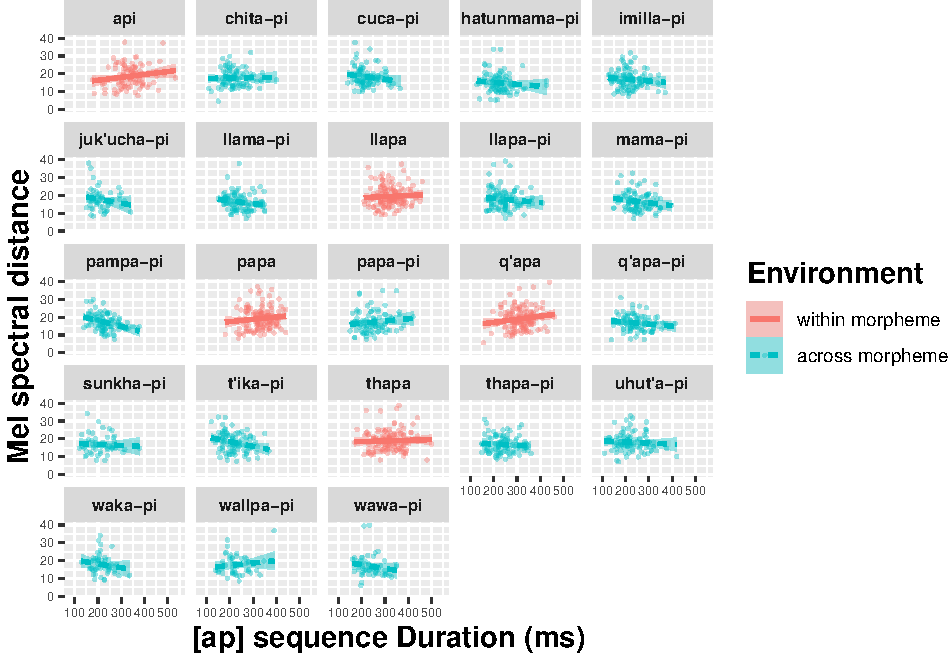
\includegraphics{3_ch3_results_files/figure-latex/child-facet-ap-word.pdf}
%\caption{\label{fig:child-facet-ap-word}Coarticulation by {[}ap{]} duration, age, and word in children}
\end{figure}


\section{Mean VC sequence duration by number of syllables in word for children}\label{app:app-G}
\begin{table}[H]
\centering
\begin{tabular}[t]{lrrrr}
\toprule
\multicolumn{1}{c}{ } & \multicolumn{2}{c}{[am]} & \multicolumn{2}{c}{[ap]} \\
\cmidrule(l{3pt}r{3pt}){2-3} \cmidrule(l{3pt}r{3pt}){4-5}
Syllables & Duration (ms) & SD  & Duration (ms) & SD\\
\midrule
2 & 272.9 & 52 & 325.3 & 57\\
3 & 211.6 & 51 & 235.2 & 51\\
4 & 207.6 & 46 & 220.7 & 51\\
5 & 204.1 & 35 & 230.4 & 51\\
\bottomrule
\end{tabular}
\end{table}

\section{Mean VC sequence duration by number of syllables in word for adults}\label{app:app-H}
\begin{table}[H]
\centering
\begin{tabular}[t]{lrrrr}
\toprule
\multicolumn{1}{c}{ } & \multicolumn{2}{c}{[am]} & \multicolumn{2}{c}{[ap]} \\
\cmidrule(l{3pt}r{3pt}){2-3} \cmidrule(l{3pt}r{3pt}){4-5}
Syllables & Duration (ms) & SD  & Duration (ms) & SD\\
\midrule
2 & 177.6 & 39 & 192.4 & 57\\
3 & 176.5 & 35 & 210.0 & 50\\
4 & 168.0 & 36 & 195.3 & 43\\
5 & 178.5 & 51 & 207.3 & 40\\
\bottomrule
\end{tabular}
\end{table}



\section{Coarticulation by sequence duration, word, and morphological environment in children}\label{app:app-I}

\begin{figure}
\centering
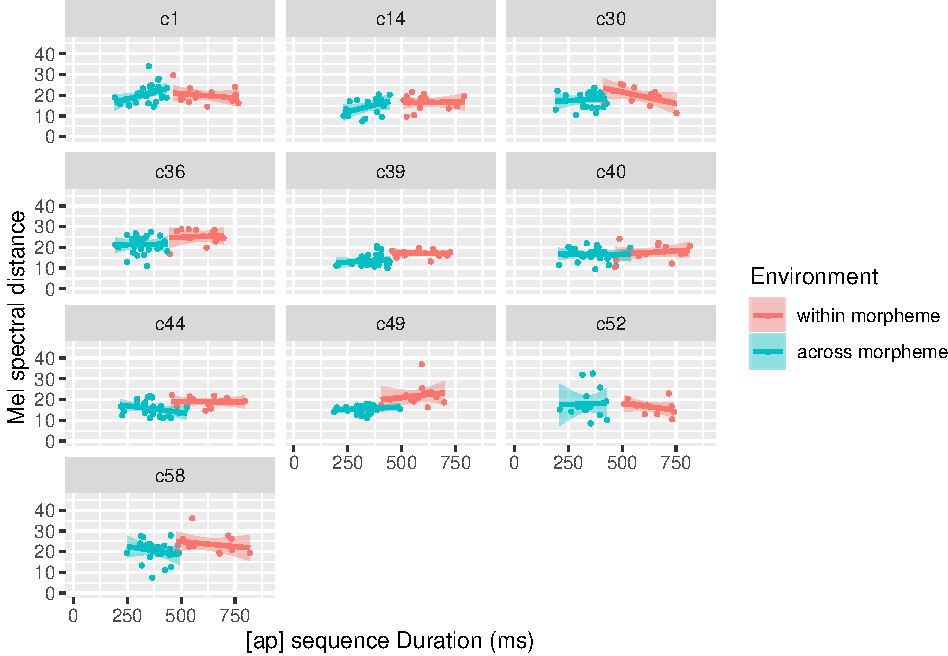
\includegraphics{3_ch3_results_files/figure-latex/five-facet-ap-1.pdf}
\caption{\label{fig:five-facet-ap}Coarticulation by {[}ap{]} duration, word, and morphological environment in five-year-old children}
\end{figure}

\begin{figure}
\centering
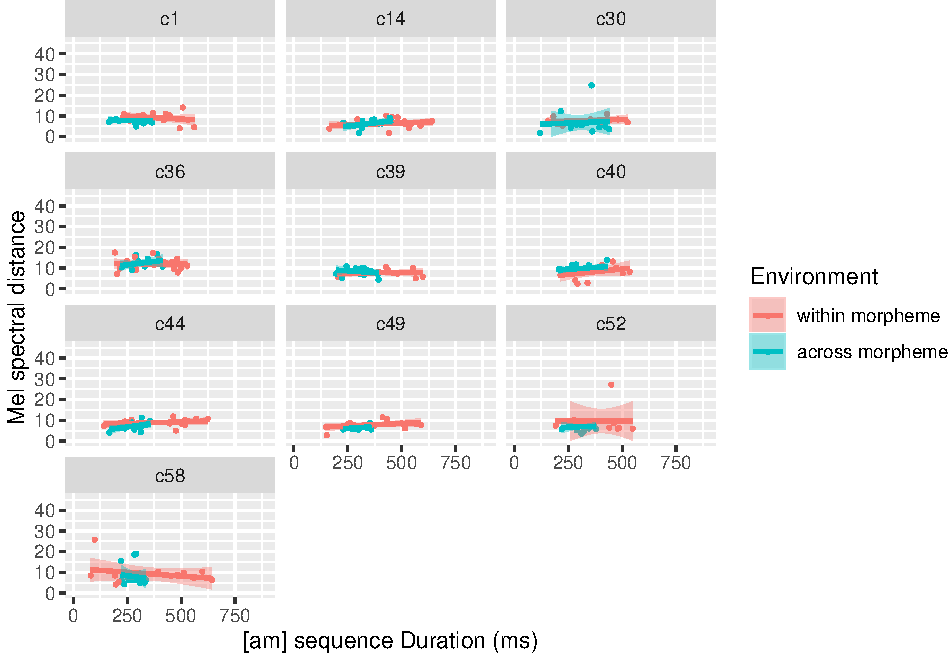
\includegraphics{3_ch3_results_files/figure-latex/five-facet-am-1.pdf}
\caption{\label{fig:five-facet-am}Coarticulation by {[}am{]} duration, word, and morphological environment in five-year-old children}
\end{figure}

\begin{figure}
\centering
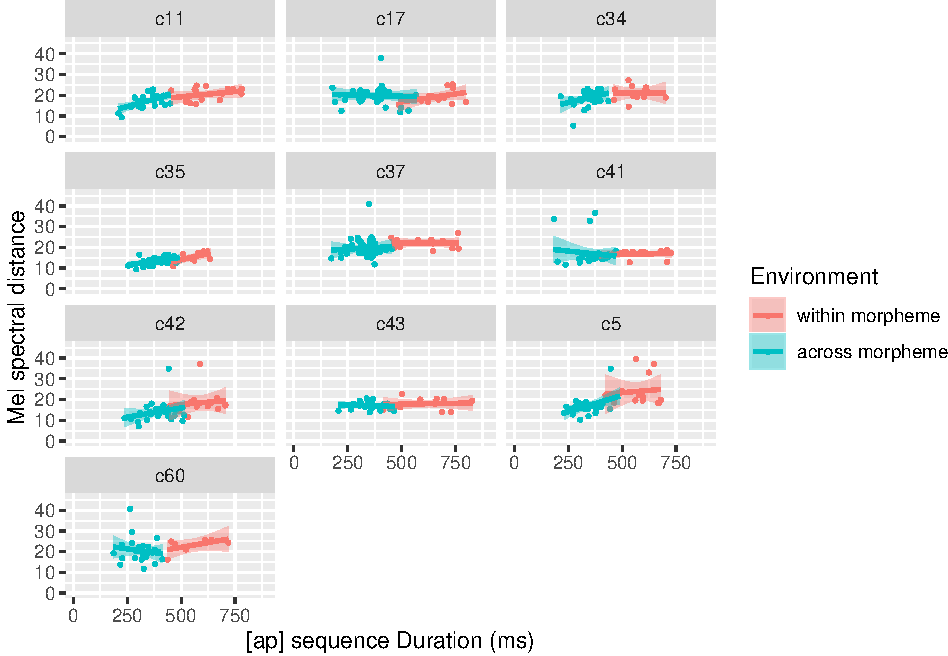
\includegraphics{3_ch3_results_files/figure-latex/six-facet-ap-1.pdf}
\caption{\label{fig:six-facet-ap}Coarticulation by {[}ap{]} duration, word, and morphological environment in six-year-old children}
\end{figure}

\begin{figure}
\centering
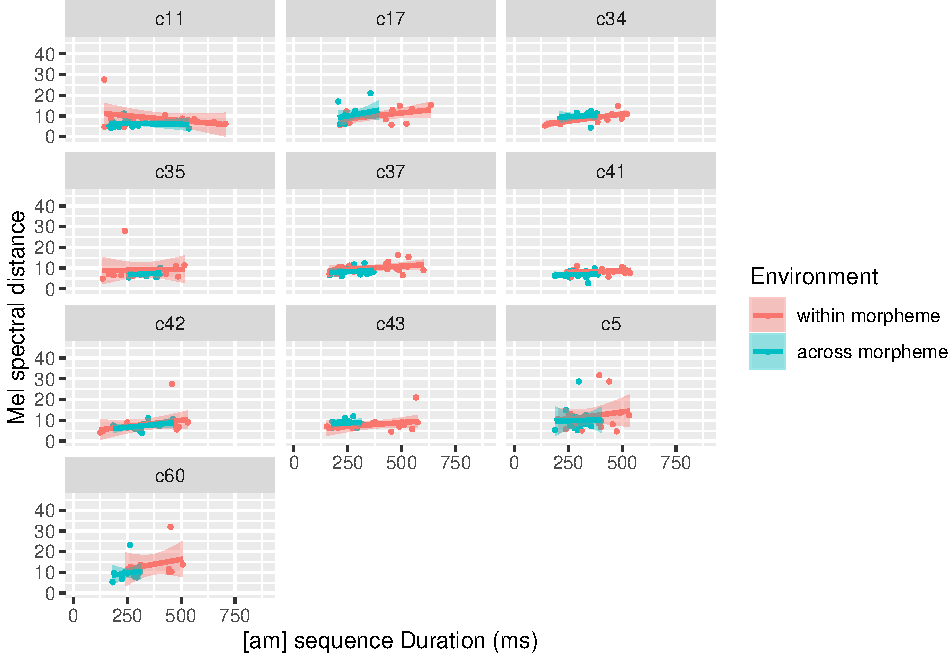
\includegraphics{3_ch3_results_files/figure-latex/six-facet-am-1.pdf}
\caption{\label{fig:six-facet-am}Coarticulation by {[}am{]} duration, word, and morphological environment in six-year-old children}
\end{figure}

\begin{figure}
\centering
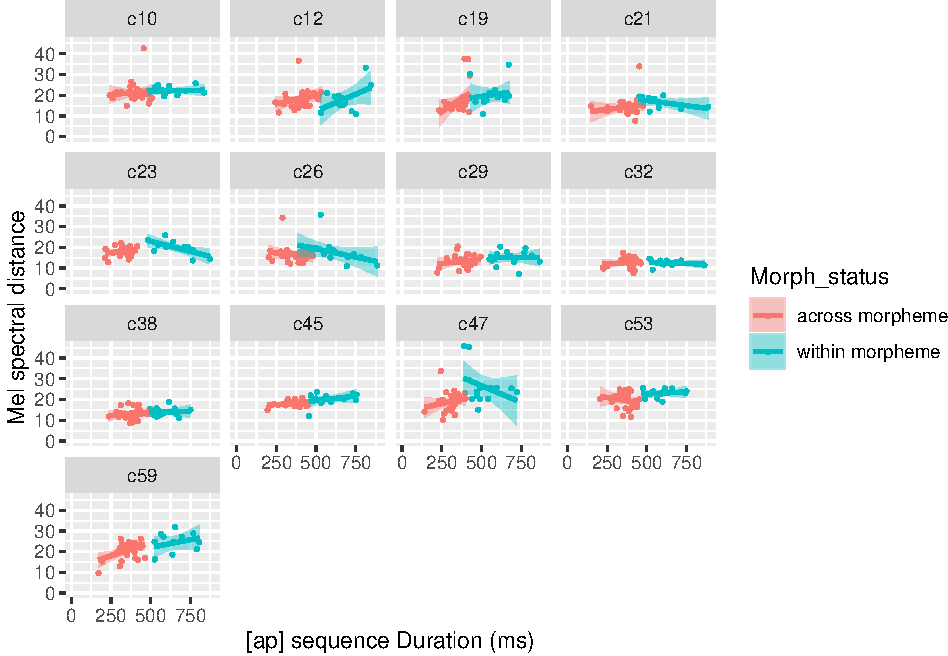
\includegraphics{3_ch3_results_files/figure-latex/seven-facet-ap-1.pdf}
\caption{\label{fig:seven-facet-ap}Coarticulation by {[}ap{]} duration, word, and morphological environment in seven-year-old children}
\end{figure}

\begin{figure}
\centering
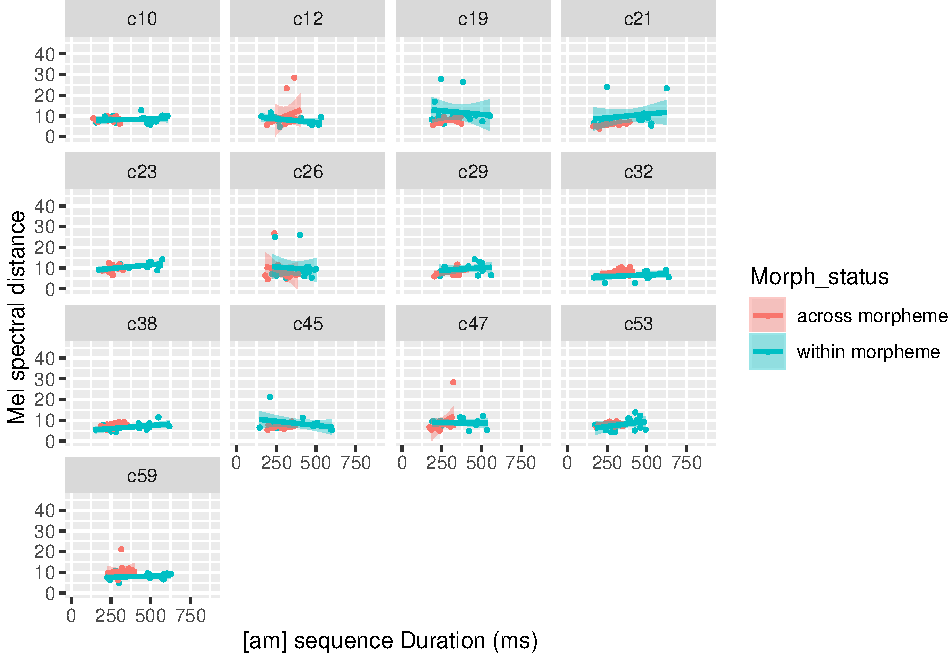
\includegraphics{3_ch3_results_files/figure-latex/seven-facet-am-1.pdf}
\caption{\label{fig:seven-facet-am}Coarticulation by {[}am{]} duration, word, and morphological environment in seven-year-old children}
\end{figure}

\begin{figure}
\centering
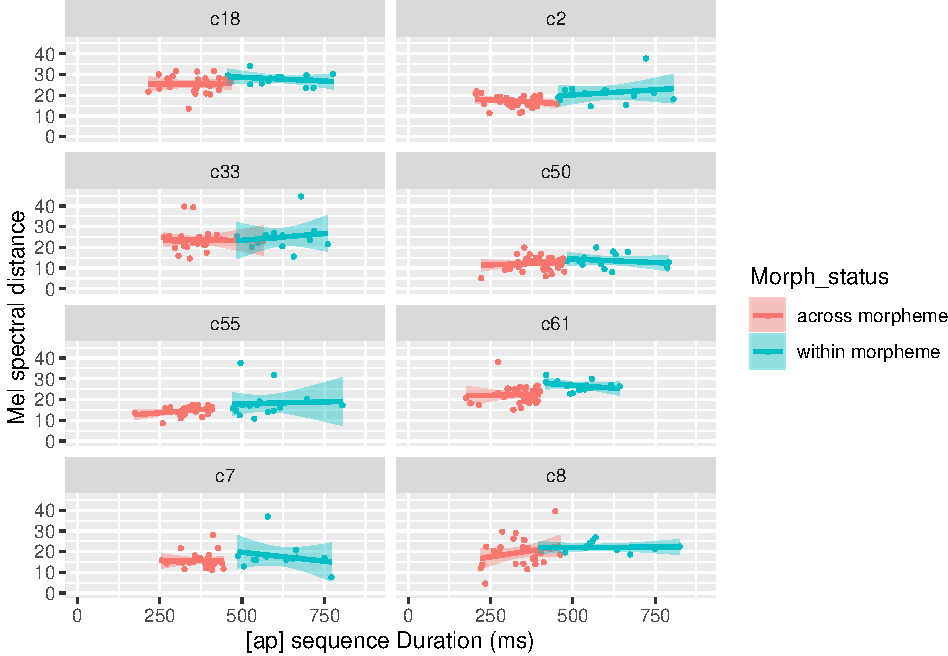
\includegraphics{3_ch3_results_files/figure-latex/eight-facet-ap-1.pdf}
\caption{\label{fig:eight-facet-ap}Coarticulation by {[}ap{]} duration, word, and morphological environment in eight-year-old children}
\end{figure}

\begin{figure}
\centering
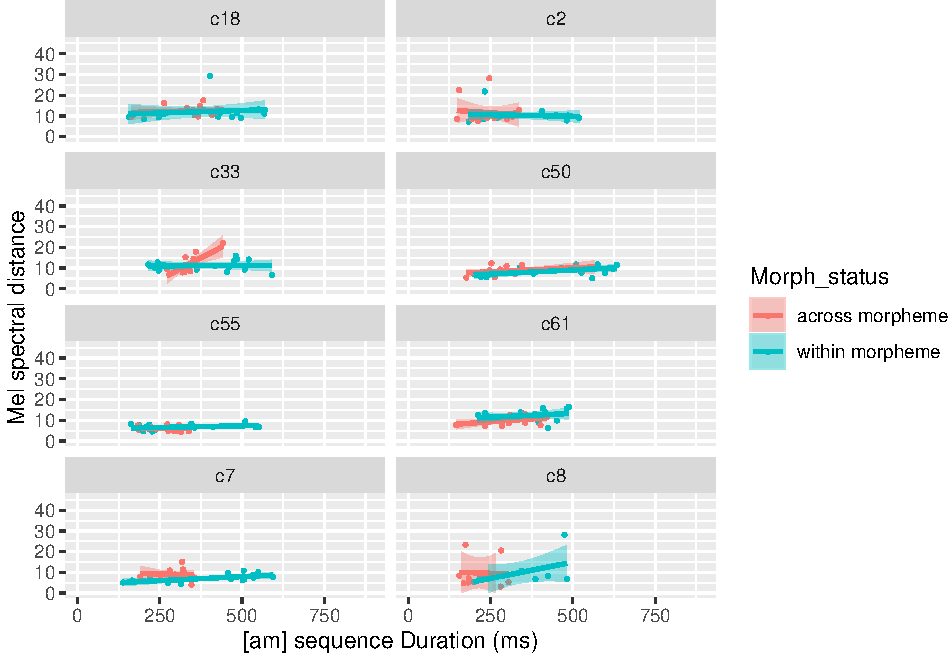
\includegraphics{3_ch3_results_files/figure-latex/eight-facet-am-1.pdf}
\caption{\label{fig:eight-facet-am}Coarticulation by {[}am{]} duration, word, and morphological environment in eight-year-old children}
\end{figure}

\begin{figure}
\centering
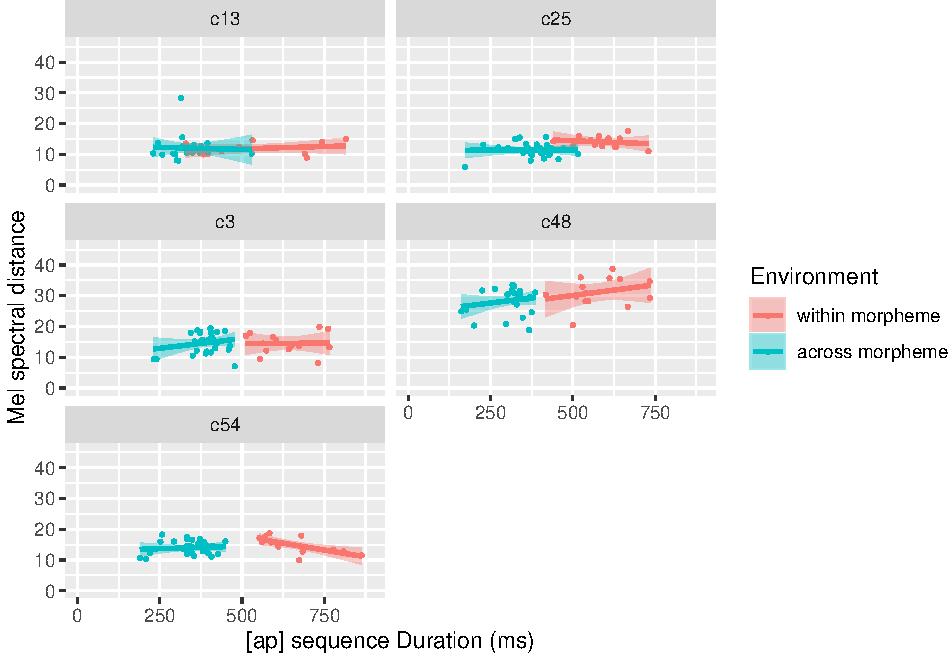
\includegraphics{3_ch3_results_files/figure-latex/nine-facet-ap-1.pdf}
\caption{\label{fig:nine-facet-ap}Coarticulation by {[}ap{]} duration, word, and morphological environment in nine-year-old children}
\end{figure}

\begin{figure}
\centering
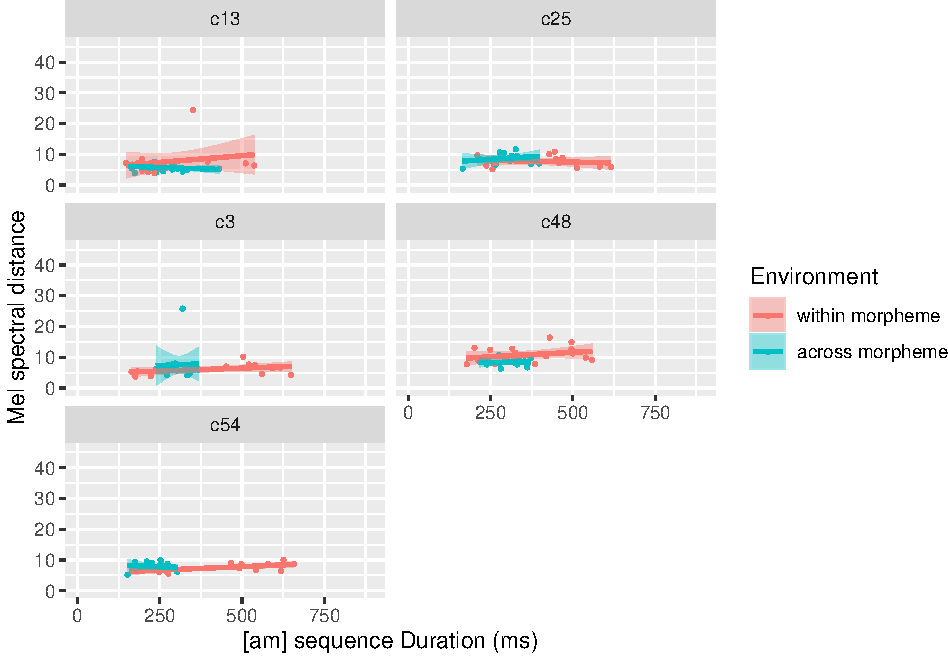
\includegraphics{3_ch3_results_files/figure-latex/nine-facet-am-1.pdf}
\caption{\label{fig:nine-facet-am}Coarticulation by {[}am{]} duration, word, and morphological environment in nine-year-old children}
\end{figure}

\begin{figure}
\centering
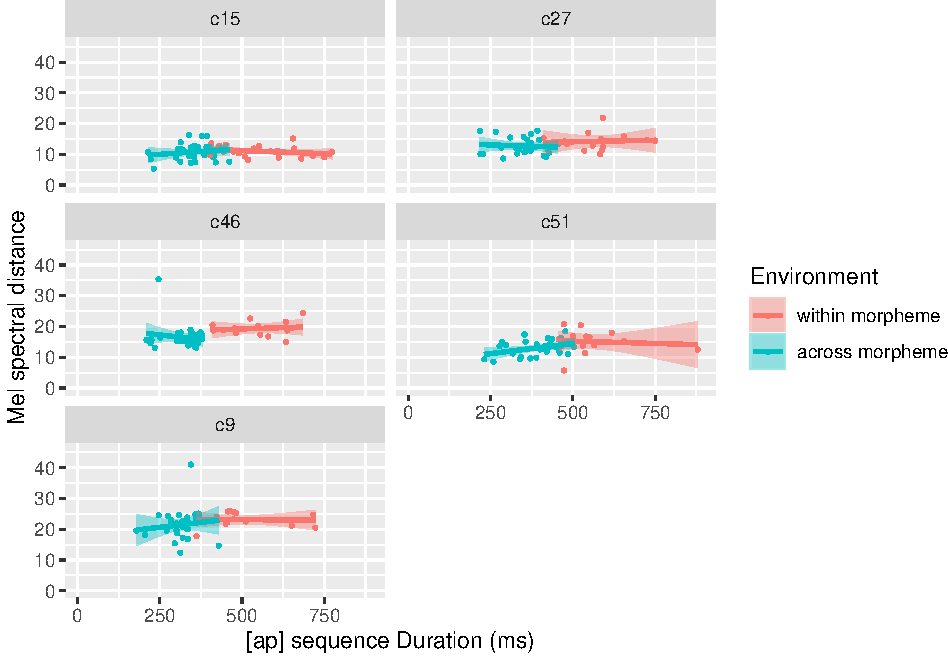
\includegraphics{3_ch3_results_files/figure-latex/ten-facet-ap-1.pdf}
\caption{\label{fig:ten-facet-ap}Coarticulation by {[}ap{]} duration, word, and morphological environment in ten-year-old children}
\end{figure}

\begin{figure}
\centering
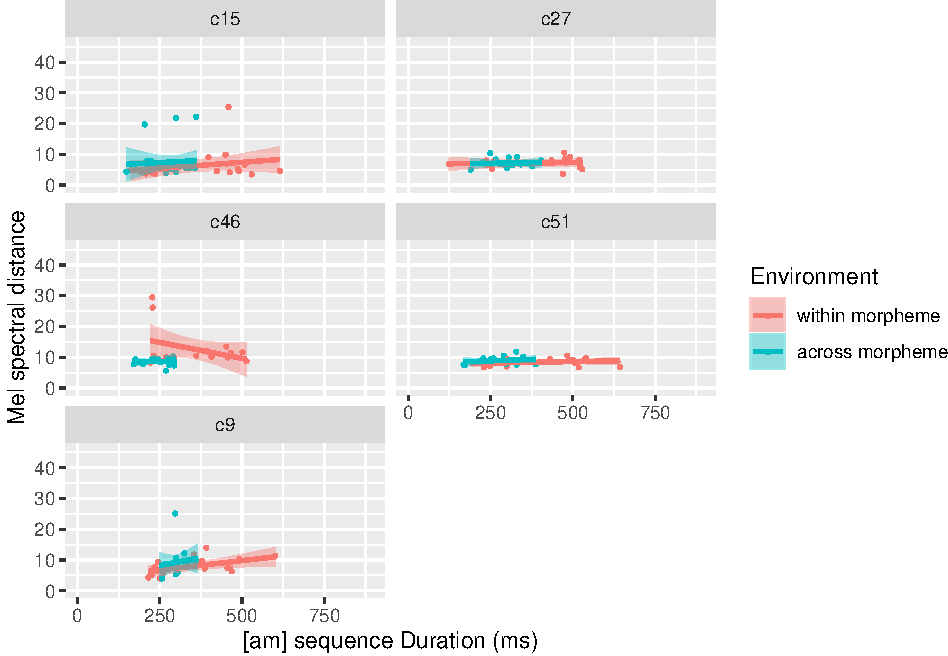
\includegraphics{3_ch3_results_files/figure-latex/ten-facet-am-1.pdf}
\caption{\label{fig:ten-facet-am}Coarticulation by {[}am{]} duration, word, and morphological environment in ten-year-old children}
\end{figure}



\end{document}


